\documentclass[11pt]{article}
\usepackage{geometry}                
\geometry{letterpaper}                   





\usepackage[english]{babel}
\usepackage[utf8x]{inputenc}
\usepackage{amsmath}
\usepackage{tikz}
\usepackage{adjustbox}
\usetikzlibrary{positioning}


\usetikzlibrary{arrows,automata}


%\usepackage[latin1]{inputenc}
\usepackage{graphicx}
\usepackage{amssymb}
\usepackage{epstopdf}
\usepackage{hyperref}
%\usepackage{natbib}
\usepackage{amssymb, amsmath}
\DeclareGraphicsRule{.tif}{png}{.png}{`convert #1 `dirname #1`/`basename #1 .tif`.png}
\title{Airplane Boarding}
\author{Anton Schäfer, Nils Blach}
%\date{date} 

\begin{document}



\thispagestyle{empty}

\begin{center}
\includegraphics[width=5cm]{ETHlogo.eps}

\bigskip


\bigskip


\bigskip


\LARGE{ 	Lecture with Computer Exercises:\\ }
\LARGE{ Modelling and Simulating Social Systems\\}

\bigskip

\bigskip

\small{Project Report}\\

\bigskip

\bigskip

\bigskip

\bigskip


\begin{tabular}{|c|}
\hline
\\
\textbf{\LARGE{Insert Title Here}}\\
\textbf{\LARGE{...}}\\
\\
\hline
\end{tabular}
\bigskip

\bigskip

\bigskip

\LARGE{Name 1, Name 2  \& [...]}



\bigskip

\bigskip

\bigskip

\bigskip

\bigskip

\bigskip

\bigskip

\bigskip

Zurich\\
Dec 2018\\

\end{center}



\newpage

%%%%%%%%%%%%%%%%%%%%%%%%%%%%%%%%%%%%%%%%%%%%%%%%%

\newpage
\section*{Agreement for free-download}
\bigskip


\bigskip


\large We hereby agree to make our source code for this project freely available for download from the web pages of COSS. Furthermore, we assure that all source code is written by ourselves and is not violating any copyright restrictions.

\begin{center}

\bigskip


\bigskip


\begin{tabular}{@{}p{3.3cm}@{}p{6cm}@{}@{}p{6cm}@{}}
\begin{minipage}{3cm}

\end{minipage}
&
\begin{minipage}{6cm}
	\vspace{2mm} \large Anton Sch{\"a}fer

 \vspace{\baselineskip}

\end{minipage}
&
\begin{minipage}{6cm}

\large Nils Blach

\end{minipage}
\end{tabular}


\end{center}
\newpage

%%%%%%%%%%%%%%%%%%%%%%%%%%%%%%%%%%%%%%%



% IMPORTANT
% you MUST include the ETH declaration of originality here; it is available for download on the course website or at http://www.ethz.ch/faculty/exams/plagiarism/index_EN; it can be printed as pdf and should be filled out in handwriting


%%%%%%%%%% Table of content %%%%%%%%%%%%%%%%%

\tableofcontents

\newpage

%%%%%%%%%%%%%%%%%%%%%%%%%%%%%%%%%%%%%%%



\section{Abstract}

\section{Individual contributions}



\paragraph{Model:} Both
\paragraph{Data Collection/Calculation:} Anton Sch{\"a}fer
\paragraph{Data Display/Graphs:} Nils Blach
\paragraph{Report:} Both

\section{Introduction and Motivations}
When it comes to air transport, efficiency is key, especially in the days of low-cost airlines. Their business models are based on using their expensive resources as efficiently as possible in order to cut cost to be able to offer cheap prices. These airlines aim to use their planes as much as possible, maximizing the time flying and minimizing turn time \footnote{The time between landing and takeoff} \cite{barrett}.

A major bottleneck for minimizing turn time is the boarding process. Between landing and takeoff, the arriving passengers have to exit the plane and, more importantly, new passengers need to enter. When entering a plane, passengers need to find their seat, store their hand luggage and sit down. During the this whole process, the passengers can only move in a narrow aisle, often obstructing each other. This can lead to long boarding times of up to thirty minutes \cite{beus}. Depending on the employed method, however, the interference between passengers can be reduced, yielding much shorter boarding times. To gain more insight on the key factors influencing the speed and efficiency of boarding, we build a model that simulates passangers' behaviour inside an airplane during boarding.

We construct our model based on information in a paper by Van Landeghem and Beuslinck \cite{beus}. In order to verify the validity of our model, we reproduce their results, and determine if our model suggests the same relationships between different boarding methods and their effectiveness.

Furthermore, we compare the performance of the boarding methods mentioned by Van Landeghem and Beuslinck and the Steffen method, a new, fast boarding method, proposed by Steffen in 2008 \cite{beus}\cite{steffen}. We simulate boarding, applying these methods on two different modern planes with different loads and measure the total and individual boarding times. Like this, we expect to gain more insight on the most relevant factors for efficient boarding and aim to verify if the Steffen method is, as expected, faster than the other methods.

Finally, we investigate the relationship between luggage amount and boarding time. Therefore, we simulate two boarding methods applied on the same airplane with luggage loads ranging from 0\% to 100 \%. We expect to see a super linear increase of boarding time, with increasing luggage load.










\section{Description of the Model}

\subsection{Overview}

Our model realistically simulates the airplane boarding process. It aims to provide reasonable information about the time required, for the seating of all passengers and individual passengers, depending on different boarding methods, luggage loads, and passenger count.  In order to achieve this, it focuses on actions taking place in the aisle, such as passengers moving, passengers storing items, and passengers moving into their seat.


\subsection{The Boarding Process}
\paragraph{At the gate.}
Before boarding, passengers usually wait at the gate. When boarding is announced, they start to line up either in random order or by group, depending on the airline or flight. Commonly used grouping schemes are either by blocks of seats, or by letter (A,B,...,F). The boarding agent announces which group is next to board the plane and the passengers enter the plane in the order of their assigned groups. Note that the order in which passengers from the same block enter the plane is random. 

\paragraph{Entering the plane.}
Passengers get to the plane via bus or through a jet bridge and enter the plane through either the front door, back door (or some middle door, if the airplane is big), or through both doors. Once inside the plane, passengers usually first try to find their seat.  Before sitting down, however, they may need to store their hand luggage. 
\paragraph{Hand luggage.} The three main types of hand luggage passengers carry are purses, backpacks and suitcases. Purses and small luggage is usually stored under the seat in front, while suitcases and large backpacks need to be put in the overhead compartments. When searching for an overhead compartment to store their items, passengers generally first check if there space in a compartment right above their seat. If it is full, they usually store their luggage in the next free compartment they see. However, passengers usually avoid walking back into the direction they came from, as this would mean going against the flow of passengers in the narrow aisle.

\paragraph{Entering seat.} After storing all their large luggage, passengers walk to their row to sit down. If noone is sitting inbetween them and their seat, they can sit down. Otherwise, the sitting passengers first have to get out of the row and let in the arriving passenger.
\\\\
Once all passengers are seated, boarding is completed.

\subsection{Our model}\label{ourmodel}

We want to gain insight on the efficiency of various boarding methods, and the impact of luggage load and passenger count on the time it takes for individuals and all passengers to board a plane. Thus, what happens in the plane is crucial, while what is taking place in the airport, jet bridge, and bus does not have significant effects on the boarding time, other than determining the order in which people arrive at the plane door. Therefore, we decide to only model the events taking place inside the airplane. To account for the impact of different boarding strategies chosen by the gate agent, we assume the passengers all enter the plane in a certain order given by their seats. We will call such an order (of seats/passengers by seat) a boarding sequence.
Although we have to keep track of which passengers are already sitting, it is not relevant what the sitting passengers are doing. Hence, for our model, we focus only on what is happening in the aisle.

We only consider airplanes with one door at the front, as all other airplanes with $n \geq 2$ doors can be divided in $n$ sections with one door. Then, boarding can simultaneously be modeled in each section individually, yielding a similar result, under the assumption, that, in reality, passengers entering the plane in one section will never enter a different section.
When choosing reasonable sections and assuming passengers behave rational, this is realistic. Similarly, we only consider airplanes with one aisle, as all other planes can again be divided into sections with one aisle each. The plane we model is configurable. Thus, our model applies to almost all airplanes.

We use an agent based model, where the actors are passengers. For simplicity, we divide the continuous time interval in discrete time steps. The actors move around in the aisle, which is a one dimensional line divided in discrete space units. Two actors can never be at the same position in the aisle, unless they are moving in opposite directions and have to pass each other. Then, they can switch positions. We model the boarding process of an actor as follows:

\paragraph{Entering the plane.}
Actors enter the plane as soon as all actors that come before them in the boarding sequence have entered the plane and if there is enough free space in the aisle for a new actor to enter. The actor then appears at the very start of the aisle.


\paragraph{Hand luggage.}
For each actor, we only consider the pieces of luggage they need to store in an overhead compartment. We discard their other luggage, as it will be stored underneath the front seat, and thus has a negligible impact on boarding time. Also, instead of taking into account every single overhead compartment, for any pair of opposite compartments, our model uses one single compartment that holds twice as many items, and covers the same space of the aisle. This simplification is realistic, as from each position in the aisle, passengers can reach the compartments on both sides. Because of this abstraction, in the remainder of this paper, when referring to a ''compartment" while speaking about our model, we mean one single big compartment corresponding to two opposite actual compartments.

	As soon as an actors can see their seat, they determine if they can store all their luggage in the comparment above their seat. If they can, they will store their luggage there, otherwise, they will store as much of their luggage as possible in the next free compartments they see. However, at first, they only move forward in order not to go against the flow. Only when they arrive at the very end of the plane and can still not store their luggage, they search for a free compartment towards the front of the plane.


\paragraph{Entering seat.}
After storing all their luggage, the actors go to their seat in order to sit down. If other sitting passengers are obstructing the way to their seat, these passengers need to move out of their seat first in order to let in the arriving actor. The arriving actor blocks the aisle during this whole time.
\\\\
Boarding is completed as soon as every actor entered their seat.






\subsection{Our Model vs. Van Landeghem's and Beuselinck's Model} 

Van Landeghem and Beuselinck produced their results ''using simulation in Arena" \cite{beus}. They modeled the boarding process similar to us, also focussing on passengers in the aisle and luggage. However, they do not explain their model precisely. Instead they state the factors they took into account:


Passengers storing luggage are a major cause for congestion in the aisle. Thus, they consider luggage, assigning each passenger a number of luggage pieces. Still, it is not clear how accurately they model luggage an compartments. In particular, we do not know if the compartments in Van Landeghem's and Beuselinck's model are defined to have a limited capacity. On one hand, they mention that, as the overhead bins fill up, ''passengers will have to move to other rows to find storage space"\cite{beus}. On the other hand, they simulate a boarding process with a full plane (with 132 seats and 23 rows) and a luggage load where 60\% of passengers carry one piece of hand luggage, 30 \% of passengers carry two pieces, and 10\% carry three. When using compartments with a realistic finite size, this should not be possible, as the total amount of luggage stored in the plane would then be:
$$ 0.6 \cdot 132 \cdot 1+ 0.3 \cdot 132 \cdot 2 + 0.1 \cdot 132 \cdot 3 = 198$$
Yet, not even a much bigger plane like the Airbus 320-200 (with 180 seats, 30 rows and space for around 110 pieces of hand luggage) provides that much space for hand luggage. We therefore assume that Van Landeghem and Beuselinck defined their compartments to have either infinite, or unrealistically large capacity. In both cases, their model does not take into account the effect of passengers who have to search for free compartments.


Furthermore, Van Landeghem and Beuselinck take into account, that, the fuller a compartment is, the longer it takes passengers to store an item in it. We decided to negelect this small extra time, assuming it will only contribute to the total boarding time as a constant summand, independent of the boarding method/sequence.


Just as in our model, they model sitting passengers having to get up in order to let someone in, if necessary. However, their model's  time values seemed unreasonable to us, so we are using different numbers. We further explain this in the section on constants.


\subsection{Constants}
Aiming to reproduce the results of Van Landeghem and Beuselinck, we defined most of our constants based the values they give in \cite{beus}:

\begin{figure}[h!]
	\center
\begin{tabular}{l|l}
	\hline
	passenger size & 25 cm \\
	\hline
	personal space & 46 cm\\
	\hline
	field of fiew & $3 \cdot$ seat pitch (lenght of a row)\\
	\hline
\end{tabular}
\end{figure}
We consider passenger size as the distance from a passengers back to their chest, which is 25 cm for the average american male, according to the NASA man-sytems integration standards \cite{nasa}. Personal space is the distance passengers will always keep from each other. We define it as one passenger size plus a 21 cm average backpack,or a jacket or suitcase.
	The passengers' field of view value is their distance to the furthest compartment they can see into and determine whether it is full already.

\begin{figure}[h!]
	\center
\begin{tabular}{l|l l l}

	&min &mode&max \\
	\hline
row enter time & 5 s &7.5 s & 15 s \\
	\hline
	row exit time& 5 s &7.5 s & 15 s \\
	\hline
\end{tabular}
\end{figure}
A passenger's row exit time is defined as the time it takes them to get up from their seat and move in the aisle. For the row exit time, we use a triangular distribution with the same constants as proposed in \cite{beus}. We define a passenger's row enter time as the time it takes them to free the aisle when sitting down \footnote{Not the time it takes them to actually sit down in their seat!} For the row enter time we use the same distribution as for the row exit time. Even if exiting a row when seated might take longer than just stepping out of the aisle, the row enter time also contains the time it takes passengers to take off their jackets, etc., so we choose the same constants as for the exit time. \footnote{Van Landeghem and Beuselinck use much higher numbers, that are not applicable to our defintion of the row enter time.}

\begin{figure}[h!]
	\center
\begin{tabular}{l|l l l}

	&min &mode&max \\
	\hline
storing time & 3 s &9.5 s & 17 s \\
	\hline

	\end{tabular}
\end{figure}
A passenger's storing time is defined as the time it takes them to store one item in an overhead compartment. We assume it is triangularly distributed, just as the constants defined in \cite{beus}. The values are based on our own observations at Zurich airport.

\begin{figure}[h!]
	\center
\begin{tabular}{l|l l l}

	&min &mode&max \\
	\hline
moving speed &0.27 m/s&0.34 s& 0.45 m/s   \\
	\hline
\end{tabular}
\end{figure}
The moving speed describes the speed at which passengers walk through the aisle. It is triangularly distributed with constants based on the values given in \cite{beus}, where it is defined as the time it takes a passenger to pass one row. When converting these time values into speed values, we assumed, that Van Landeghem and Beuselinck were referring to an airplane with a seat pitch (length of a row) of 0.813 m, which was very common for airplanes used around the year 2002, when their paper was published. Still, in our opinion, the speeds seem a bit slow.


\subsection{Boarding Methods}
A boarding method defines the order in which the passengers enter the plane, depending on their assigned seat. It does not have to specify an exact sequence of passengers, but may instead describe an order in which certain groups of passengers enter the plane. Passengers in the same group may board the plane in any order. 


As can be seen from our results, different boarding methods can lead to significantly different boarding times. Thus, when aiming to ensure quick boarding- and turn times, choosing an effective boarding method is crucial. In this paper, we analyze the effectiveness of a variety of different boarding methods given in \cite{beus}, as well as the ''Steffen" method, which was proposed by Steffen \cite{steffen} in 2008 and is supposed to be the best known boarding method as of today.



In this section, we describe the Steffen method in detail, but only provide a brief overview of the other methods, which are explained thoroughly in \cite{beus}. These explanations will be cited in the appendix. Note that, when talking about boarding methods, we can use the terms ''seat" and ''passenger" interchangeably; the passengers are ordered by their assigned seat, so any order of passengers can also be seen as an order of seats and the other way around.


\subsubsection{The Alternation Concept}

All boarding methods generally order the seats from back to front, for obvious reasons. Yet, some of them specify a parameter called alternation in their name's suffix. The alternation parameter specifies, how many groups/seats are skipped in each step, when ordering from back to front. If the alternation parameter is 0, the method orders the specific groups in descending order (e.g. 7,6,5,4,3,2,1 assuming groups with low indices are further front) and the method's suffix is ''des". For a higher alternation parameter $n$, the method also orders the groups in descending manner, taking only every $(n+1)$-th group, then repeating this process with the groups that are left (e.g. 7,4,1,6,3,5,2 for an alternation of 2). A group with an alternation parameter $n \geq 1$ has the suffix ''alt\_$n$".



\subsubsection{Description of Boarding Methods}

\paragraph{Random.} Does not specify any order. Passengers may board in any sequence.
\paragraph{by\_block.} Groups the seats into equally sized blocks where each block contains all seats of one or more rows. ''by\_block\_$n$\_$\dots$" 
divides the plane into $n$ blocks.
\paragraph{by\_halfblock.} Groups the seats into blocks, where each block contains all seats of one or more rows on only a single side of the aisle. Not that the blocks are not equally sized, if the airplane has more seats on one side of the aisle than on the other. ''by\_halfblock\_$n$\_$\dots$" divides the plane into $2\cdot n$ blocks.

\paragraph{by\_row.} Groups together all seats of one row. For obvious reasons, all ''by\_row" methods order the rows from back to front in some way (with/without alternation).

\paragraph{by\_halfrow.} Groups together all seats of one row that are on the same side of the aisle. Otherwise it is similar to ''by\_row".

\paragraph{by\_letter.} Groups together all seats with the same letter i.e. all seats in the same column.

\paragraph{by\_seat.} Defines an order on all seats. The order in which passengers board the airplane is totally defined and not random. For obvious reasons, all ''by\_seat" methods order the seats from back to front in some way.

\paragraph{Steffen.}
The Steffen method also specifies a total order on all all seats. It makes passengers board from back to front, from window to aisle, with an alternation of 1. So at first, every second seat in a column at the window (usually F) is boarded, then every second seat in the other window column (usually A). Secondly, the remaining seats from the two window columns are filled. The same process then continues with the columns second closest to the window, and so on. Figure \ref{fig:steffen} shows how the Steffen method would be applied in a plane with 7 rows and 4 seats per row.


We also measure the performance of sightly modified Steffen methods with increased alternation. ''steffen\_alt\_$n$" refers to a modified Steffen method with an alternation of $n$.

\begin{figure}
	\center
	\label{fig:steffen}
	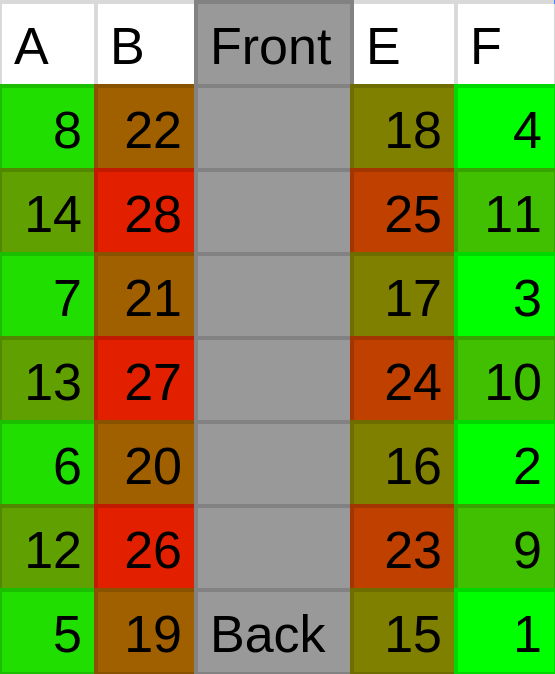
\includegraphics[width=0.3\linewidth]{images/steffen.png}
	\caption{The Steffen Method}
\end{figure}



\section{Implementation}

We implemented our model in Python. We use 0.01 m as the fundamental space unit, and 0.1 s as the fundamental time unit. The plane is implemented such that all its relevant parameters (such as number of rows, row size, seat pitch and length and size of a compartment) can be adjusted. The aisle is represented by an array, where each entry is an integer, indicating, which actor currently covers the corresponding millimeter, or if it is free. In every time step, we make every actor, that is currently in the aisle, act. When acting, actors can update their own state or the occupation of a compartment, the aisle, or their seat. Once  all actors are seated, the simulation ends, as boarding is completed.

\subsection{The Different Boarding Methods}
We generate the boarding methods as permutations of a list of all seats in the plane. Then, each actor gets assigned one of the seats and the actors enter the plane in the order of the permuted list of seats. Random seats are deleted from the list, if the plane is not fully loaded.

\subsection{Acting and Actor States}
\begin{figure}[h!]
	\center
\begin{tabular}{|ll|l|}
	\hline
	State & &Description\\
	\hline
0 &     & not yet in plane                        \\
\hline
1 & 1/0 & looking for storage room by seat        \\
  & 1/1 & looking for storage room behind seat    \\
  & 1/2 & looking for storage room further front  \\
  \hline
2 & 2/0 & storing luggage (coming from state 1/0) \\
  & 2/1 & storing luggage (coming from state 1/1) \\
  & 2/2 & storing luggage (coming from state 1/2) \\
  \hline
3 &     & going to seat                           \\
\hline
4 &     & sitting down                            \\
\hline
5 &     & sitting in seat       \\                 
\hline

\end{tabular}
\caption{Actor states}
\label{tab:states}
\end{figure}

\begin{figure}[h!]

%	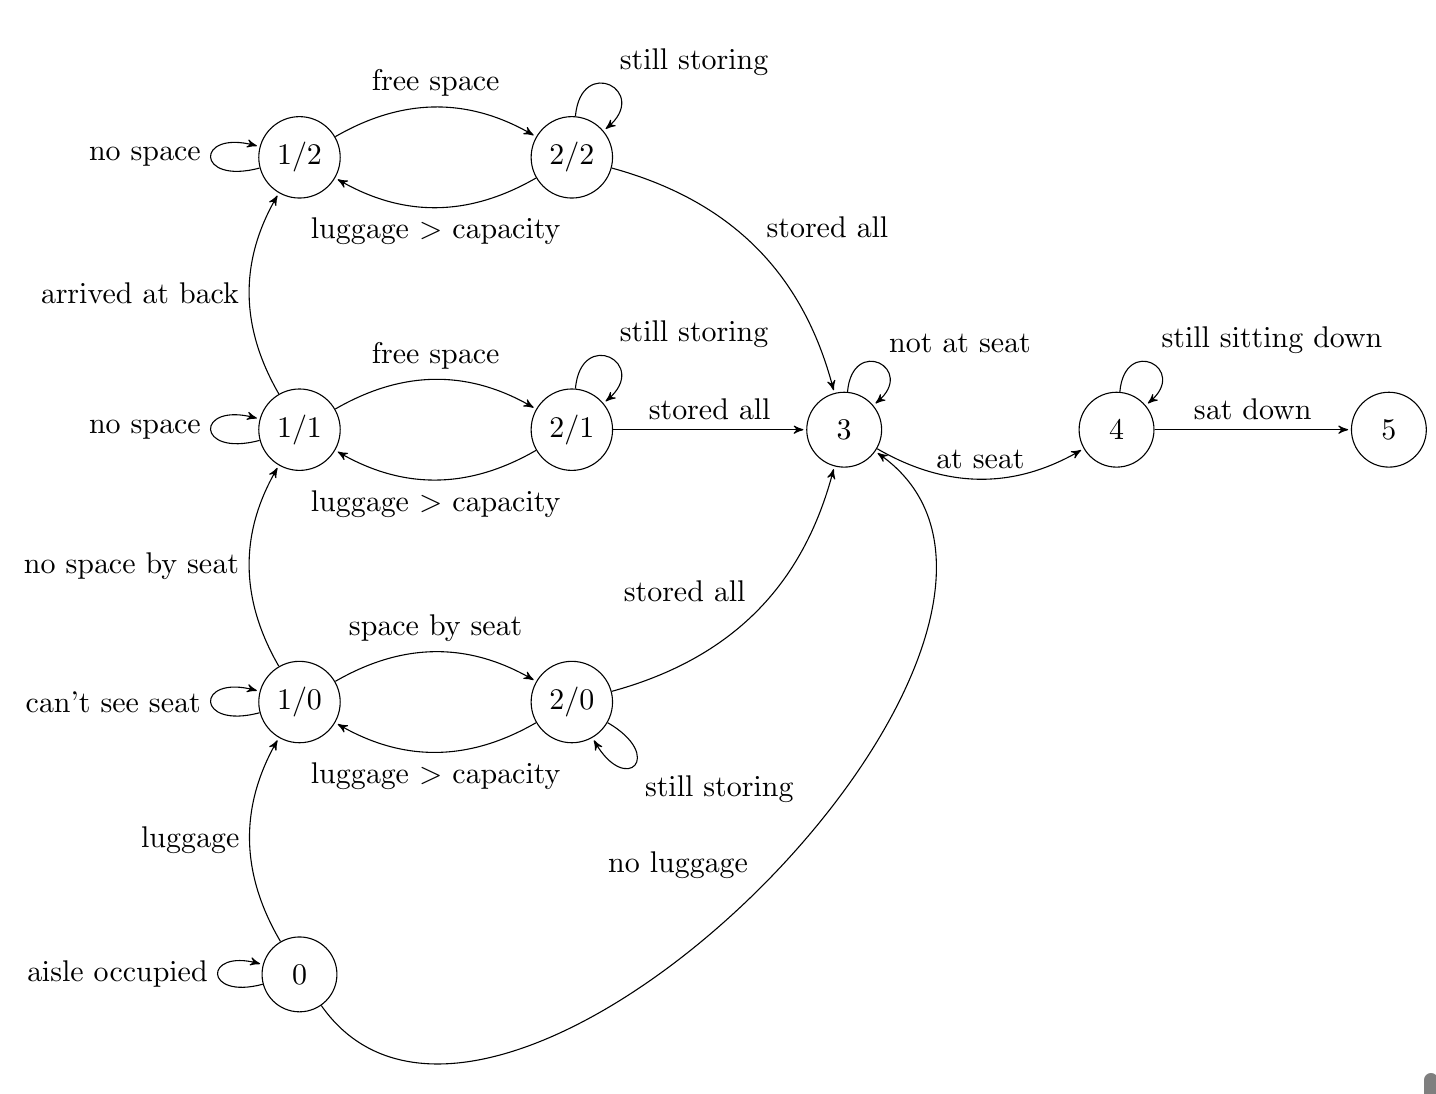
\includegraphics[width=\linewidth]{images/fsm.png}
%	\label{fig:fsm}
	\caption{The actor finite state machine}
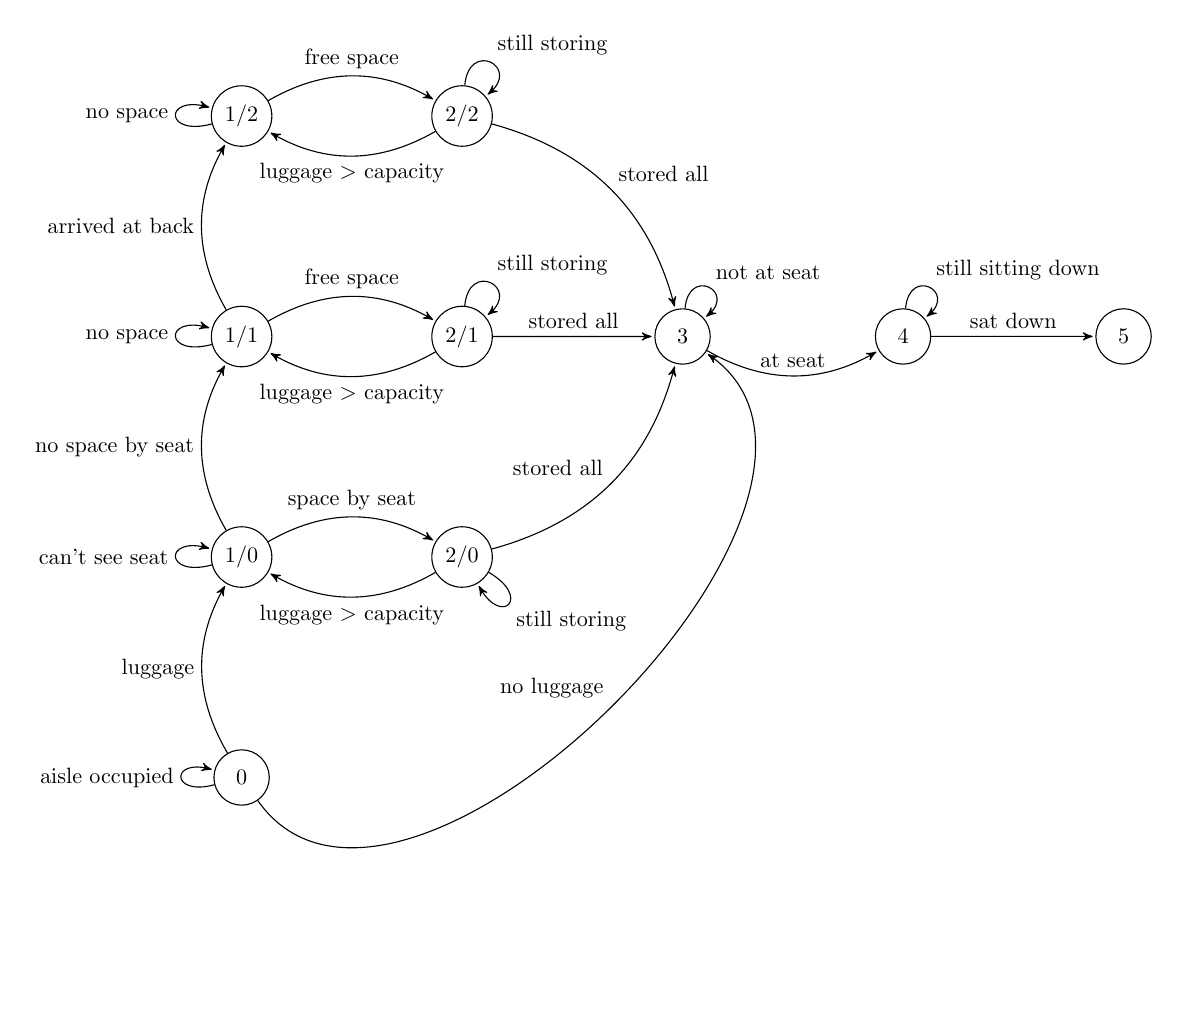
\begin{tikzpicture}[->,>=stealth',shorten >=1pt,auto,node distance=3.5cm,
        scale = 0.8,transform shape]

\node[state] (0) [] {$0$};
 \node[state] (1/0) [above of=0] {$1/0$};
 \node[state] (1/1) [above of=1/0] {$1/1$};
 \node[state] (1/2) [above of=1/1] {$1/2$};
 \node[state] (2/0) [right of=1/0] {$2/0$};
 \node[state] (2/1) [right of=1/1] {$2/1$};
 \node[state] (2/2) [right of=1/2] {$2/2$};
 \node[state] (3) [right of=2/1] {$3$};
 \node[state] (4) [right of=3] {$4$};
 \node[state] (5) [right of=4] {$5$};

 \path (0) edge   [bend left]           node {luggage} (1/0)
       (0) edge  [bend right=100]            node {no luggage} (3)
       (0) edge  [loop left]            node {aisle occupied} (0)
       (1/0) edge  [loop left]            node {can't see seat} (1/0)
       (1/0) edge    [bend left]          node {no space by seat} (1/1)
       (1/0) edge   [bend left]           node {space by seat} (2/0)
       (1/1) edge  [loop left]            node {no space} (1/1)
       (1/1) edge   [bend left]           node {arrived at back} (1/2)
       (1/1) edge   [bend left]            node {free space} (2/1)
       (1/2) edge   [loop left]           node {no space} (1/2)
       (1/2) edge    [bend left]           node {free space} (2/2)
       (2/0) edge     [out=330,in=300,looseness=8]        node {still storing} (2/0)
       (2/0) edge    [bend left]          node {luggage $>$ capacity} (1/0)
       (2/0) edge     [bend right]         node {stored all} (3)
       (2/1) edge      [out=85,in=40,looseness=5]        node {still storing} (2/1)
       (2/1) edge     [bend left]         node {luggage $>$ capacity} (1/1)
       (2/1) edge              node {stored all} (3)
       (2/2) edge     [out=85,in=40,looseness=5]         node {still storing} (2/2)
       (2/2) edge     [bend left]         node {luggage $>$ capacity} (1/2)
       (2/2) edge     [bend left]         node {stored all} (3)
       (3) edge     [out=85,in=40,looseness=5]       node {not at seat} (3)
       (3) edge     [bend right]         node {at seat} (4)
       (4) edge      [out=85,in=40,looseness=5]         node {still sitting down} (4)
       (4) edge              node {sat down} (5);

\end{tikzpicture}
\label{fig:fsm}
\end{figure}

Actors behave like finite state machines. They can be in 10 different states, and transition from state to state based on certain conditions. These states can be seen in figure \ref{tab:states}. Figure \ref{fig:fsm} shows the actor as a FSM and gives an overview over how actors behave.

\paragraph{(0) Entering plane.} All actors start in state 0, waiting on their turn to enter the plane. Once it is their turn to enter the plane, and there is enough free space in the aisle, they mark the aisle space they cover as occupied and thereby enter the plane. Then, they either update their state to state 1 or state 3, depending if they carry any hand luggage or not. From now on, their method act will be called in every time step until they are seated.

\paragraph{(1) Finding space.}
There are three sub states of state 1. When transitioning into state 1, actors land in the sub state 0 (1/0), where they are looking for free compartment space by their seat. As soon as the distance of their position to their seat is less than their field of view, they either transition to state 1/1, if it cannot hold all their luggage or stay in state 1/0, walking towards their seat. When there is still space by their seat once they arrive, they store their items, transitioning to state 2/0.

When in state 1/1 actors are searching for any free space further back the aisle. They advance until they either find a free compartment and start to store, transitioning to state 2/1, or reach the very end of the plane and transition to state 1/2.

In state 1/2 actors are walking towards the front of the plane, searching for a free compartment. As soon as they find free space, they transition into state 2/2 in order to store their items.

\paragraph{(2) Storing luggage.}
When starting to store luggage, actors immediately mark the space their luggage takes up in the respective compartment as occupied. They then stay in this state for a number of time steps, corresponding to their storing time multiplied with the number of pieces they are storing. After finshing storing as much items as they could, they transition to state 3, in order to sit down, if they successfully stored all their hand luggage. Otherwise, the compartment could not hold all their luggage, so they transition back to state 1 (from 2/$i$ into 1/$i$ for $i \in \{0,1,2\})$ to find another free compartment.

\paragraph{(3) Going to seat.}
When going to their seat, passengers just advance into the direction of their seat until they are at the right position to enter their row. Then, they transition to state (4).


\paragraph{(4) Moving into seat.}
Before being seated, actors stay in state 4 for a number of timesteps, corresponding to their row enter time plus the row exit times of all passengers already sitting between them and their seat. Only after remaining in state 4 for this amount of time, blocking the aisle, they can transition into state 5.

\paragraph{(5) Seated.}
Once an actor is seated, his state will never change again. Even when moving out of the seat, in order to let in another passenger, seated actor's states are not updated. Still, seated actors can have an influence on other passengers, as can be seen in the description of state 4.


\subsubsection{Moving and Switching}
When moving forward or backward, in one timestep, actors can move as far as their moving speed allows them. However, when the aisle is occupied by another actor, they cannot move further. Instead, they determine, if the actor blocking the aisle wants to move into the opposite direction of their goal. If this is the case, in order to advance, the two passengers can switch positions. When two passengers switch positions, the space they occupy in the aisle cannot be entered by any other actor. Yet, in this space, the two can move freely, possibly overlapping positions. However, the two can only move at half their normal speed, as they need to pass each other in the narrow aisle. After they finished switching postions, or after one of them sat down, the switching process can be ended. Then, both actors are at different positions again, and other actors may now enter the previously blocked space.





\subsection{Graphics and Calculation}
Our model also provides animations for the boarding process, which can be displayed after the whole simulation has been calculated. These can be useful, when one wants to gain more insight on what happens under the hood of the simulations/model, or if one tries to understand how, or why, a specific boarding method yields certain results.

 



\section{Simulation Results and Discussion}
\begin{figure}
	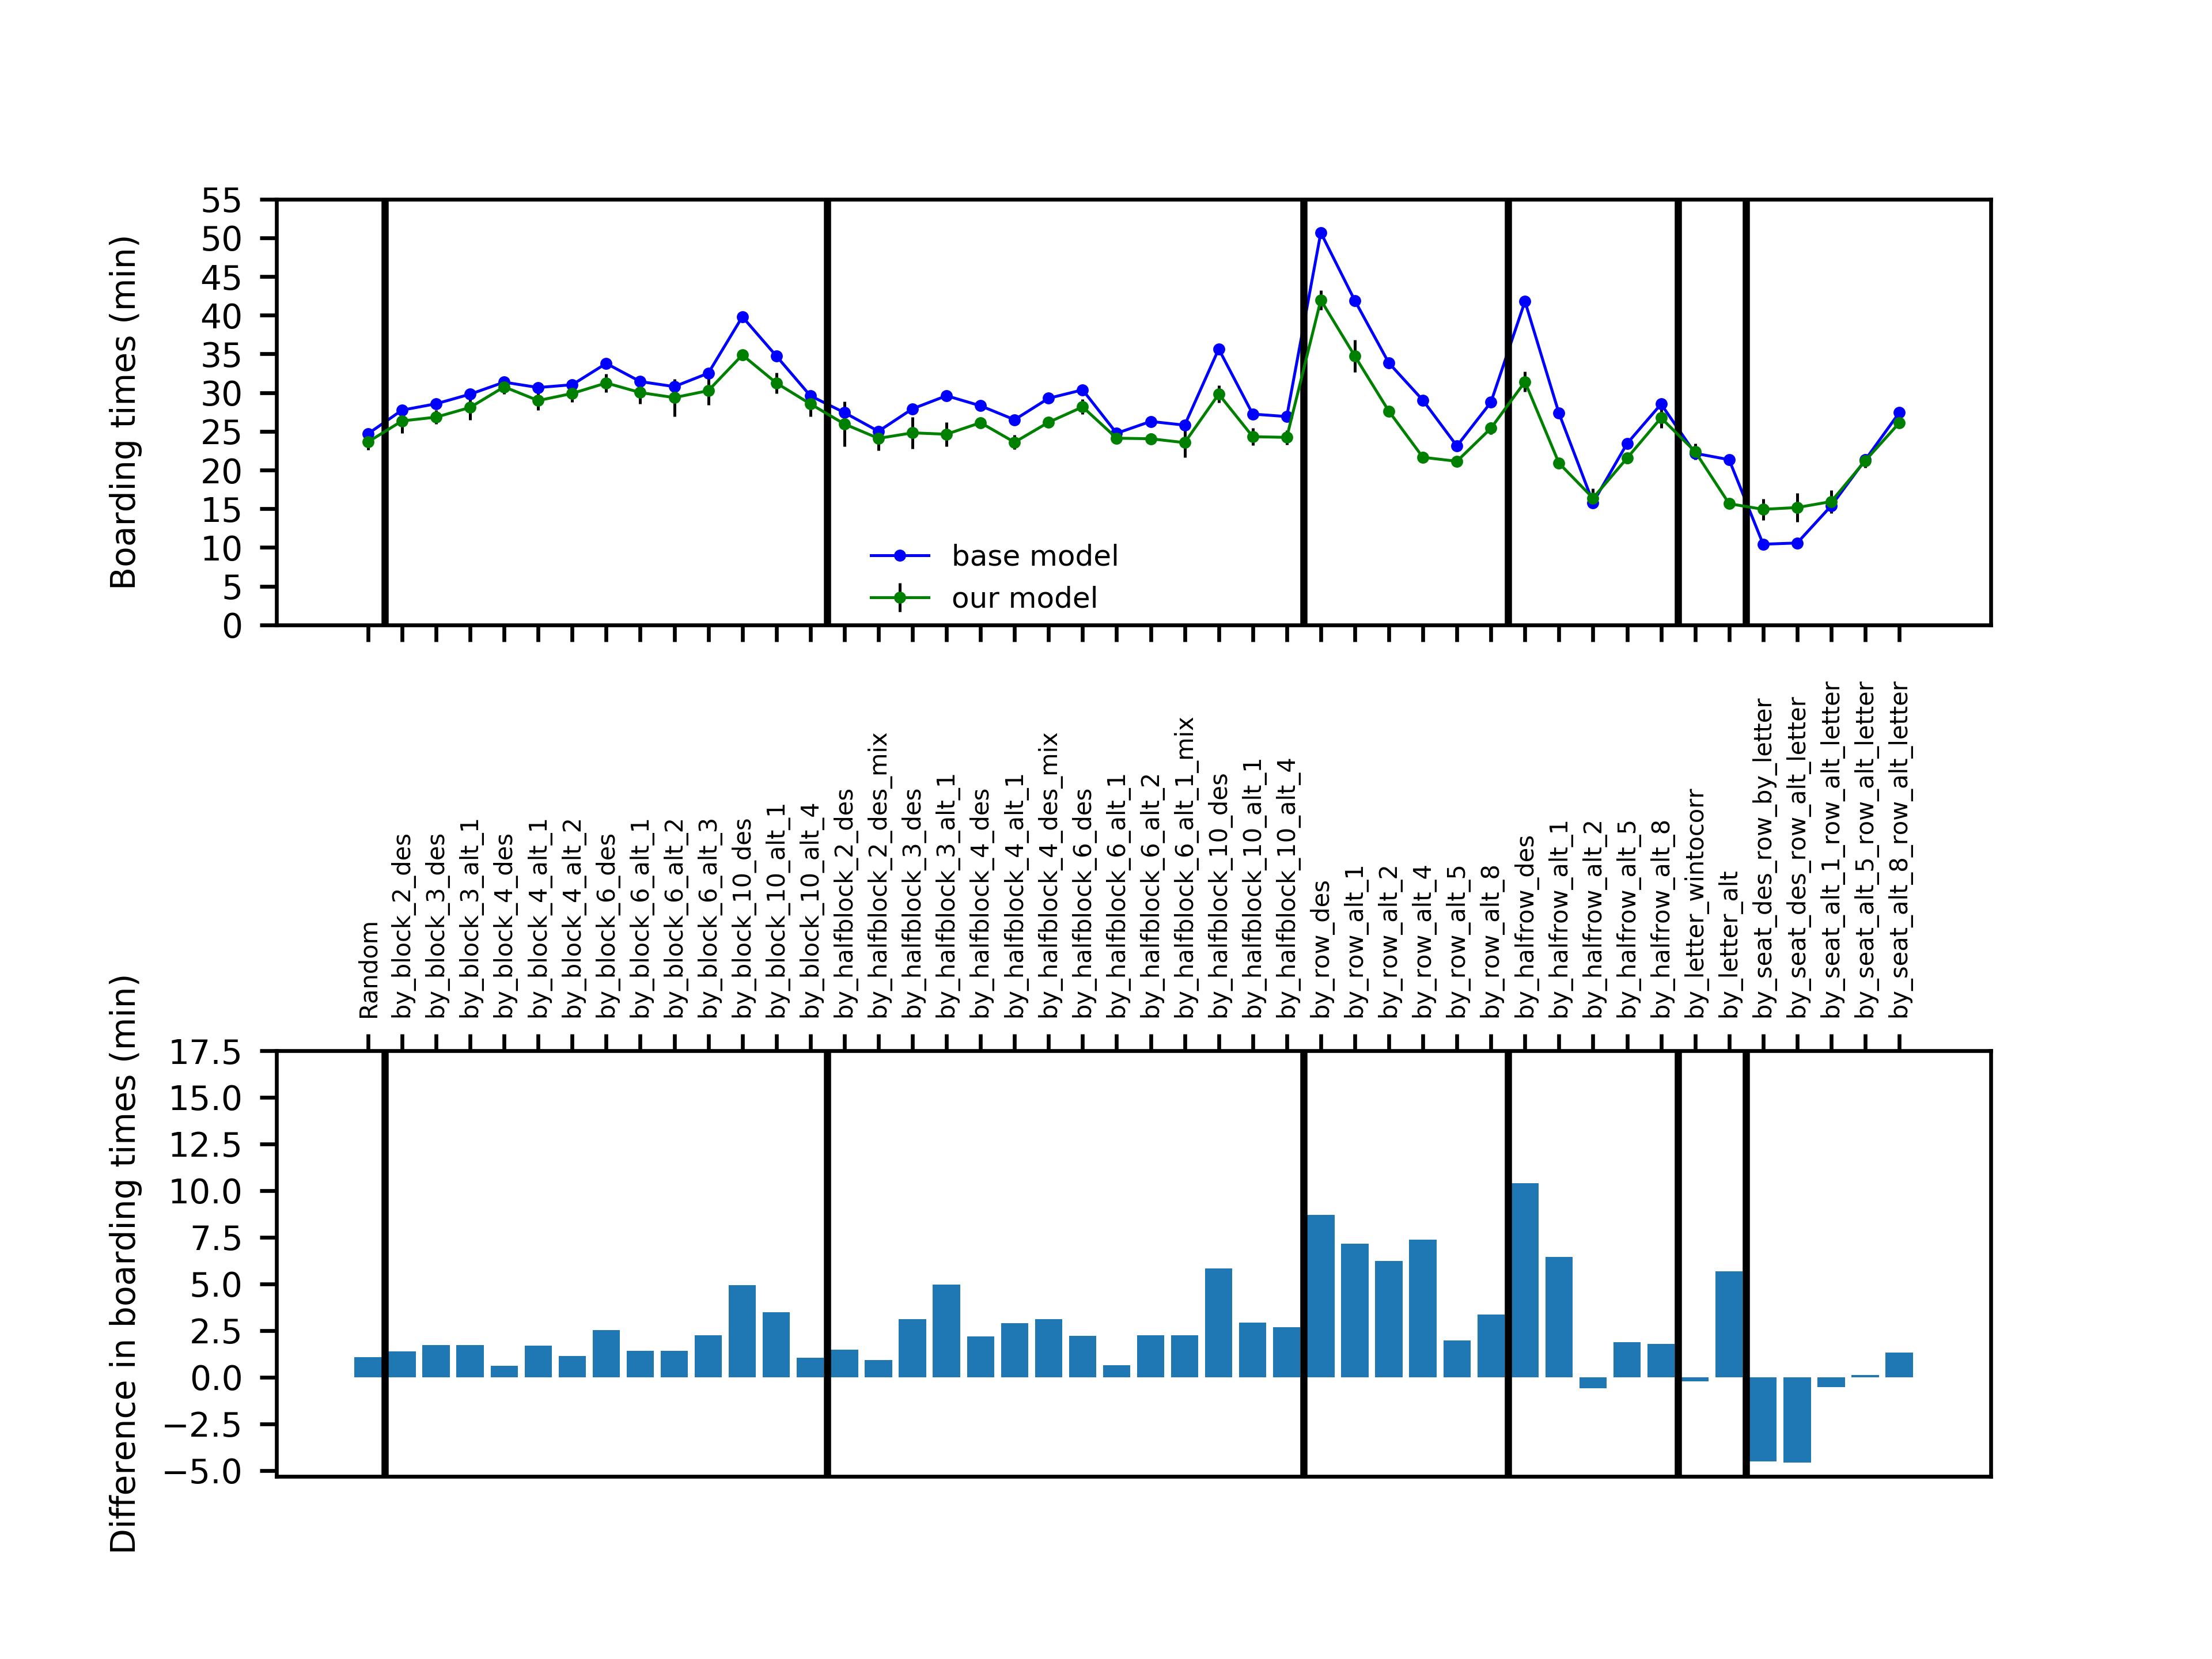
\includegraphics[width=\linewidth]{../../code/AirplaneBoarding/data/figure1/figure1.png}
	\caption{This figure compares the results from our model, using a similar airplane and load specifications, to the ones from the model used by Van Landeghem and Beuselinck.}
	\label{figure1}
\end{figure}
\subsection{Result Comparison - Our model vs. Van Landeghem's and Beuselinck's Model} \label{model_comp}
In order to validate the correctness of our model we compare the different boarding times resulting from employing the same boarding methods as was done in \cite{beus} with a similar airplane (around 2002) and load level. The airplane used in both models are equivalent in the number of rows they have (23) and the number of seats in each row (6), with the only minor exception that the plane they used only had 3 seats in the first and last row. However this difference is very minor, so we decided to neglect it. The passenger load level, so the percentage of occupied seats in the aircraft, are in both cases identical at $100\%$. Furthermore the luggage load level in the simulation from Van Landeghem and Beuselinck was set to normal, which we had to translate into the percentage of occupied overhead compartment space, as our model handles luggage differently to theirs. We believe that when the plane is completely booked out, it is reasonable to assume that $90\%$ of available overhead compartment space is occupied with a normal load level.

In total for each of the 46 boarding methods used in \cite{beus}(excluding method ''by\_block\_B-E" because it differentiates with business class in addition to economy class, which, for given reasons, we don't do) we performed 5 trials, in order to have a small sample to calculate the mean time taken for each one within a $95\%$ confidence interval.
The results for the confidence intervals of the total boarding times and differences to Van Landeghem's and Beuselinck's results (their minus our) are displayed in Figure \ref{figure1}, which is divided into two subplots. The plot at the top shows for each method the average boarding time in minutes with a 95\% confidence interval (error bars) and the plot at the bottom the differences in results (Van Landeghem's and Beuselinck's minus Our). The vertical black lines divide the different boarding methods into their respective classes. The blue data is from the ''base model" from \cite{beus} and the green from our model. For numerical values, please check table \textit{Insert reference here} in the Appendix. 
Analysing the results lead to following conclusions:


The first conclusion that can be drawn is that the average boarding times for our model are generally lower with only a few exceptions. This phenomenon is most likely caused by the different ways the two models handle luggage. In our model the time it takes to store luggage inside a specific compartment does not increase with the amount of luggage that is already inside, which is the case for the other model. Furthermore, not everyone necessarily has any luggage with them because the number of actors (138) is much larger than the total amount of hand-luggage (75) distributed between them (no one more than 2 pieces), which means there are plenty which can directly move to their seat. In the case of the other model, every actor has between 1 and 3 pieces of luggage, so in total almost at least twice the amount of carry-on luggage and there is no one without any. These two aspects further support the observed results. On the other hand, compartments can be full, not allowing any more actors to store any of his carry-on inside of it, which means those actors have to find other free spots, which takes time and can cause interferences.  As mentioned earlier, it is not entirely clear whether the other model implements this possibility. To what extend each of these aspects impacts the result can not be said as we have not enough information about the model used in \cite{beus}. 
	
The two exceptions to this observations occur in the class ''by\_seat", but only with the two that do not alternate between rows. The reason for that is most likely that the actors in our model first always try to store their luggage in the overhead compartment above their seat and if possible start storing at the beginning of it, not allowing the actor behind to access the same compartment. So if actors that are right behind each other in the boarding sequence have seats in the same or adjacent rows, they might obstruct one another when they both have hand-luggage. This is would also explain why the exception is only seen in the two methods within class ''by\_seat" that do not alternate between rows, so adjacent actors in the boarding sequence have adjacent rows. This attribute of the actors only negatively impacted the difference in time in one class because in all the others we look at larger groups, which are random within, and not at individual seats and arrange those. Because the exception to the phenomenon, that the times of our model are generally lower, only occurs in those two methods and is caused by something reasonable, the validity of our model is not impacted. 

Now, in order to be able to conclude that our model is at least as valid as the one used by Van Landeghem's and Beuselinck's, we need to evaluate the impact that the found phenomenon has and whether its cause is justifiable. 
The general trend of the data is retained by our model because within each class, especially the larger ones, the difference in boarding times is fairly constant, which again can be seen in the bottom diagram of Figure \ref{figure1}. Furthermore, the overall relationships between boarding methods are generally preserved. So, for example, whenever the relationship between the boarding times of two adjacent methods in the ''base model"(in Figure \ref{figure1}), is positive/negative (the blue line has gradient greater/smaller zero), then the relationship between the methods in our model are also positive/negative (the green line also has a gradient greater/smaller zero). For those reasons and the ones justifying the assumptions we made in section \ref{ourmodel}, we believe that there is enough reason to safely assume that our model realistically simulates reality using a certain level of abstraction.  

\subsection{Comparison of different boarding methods - Bombardier CS100 \& Airbus A320-200}
\begin{figure}
	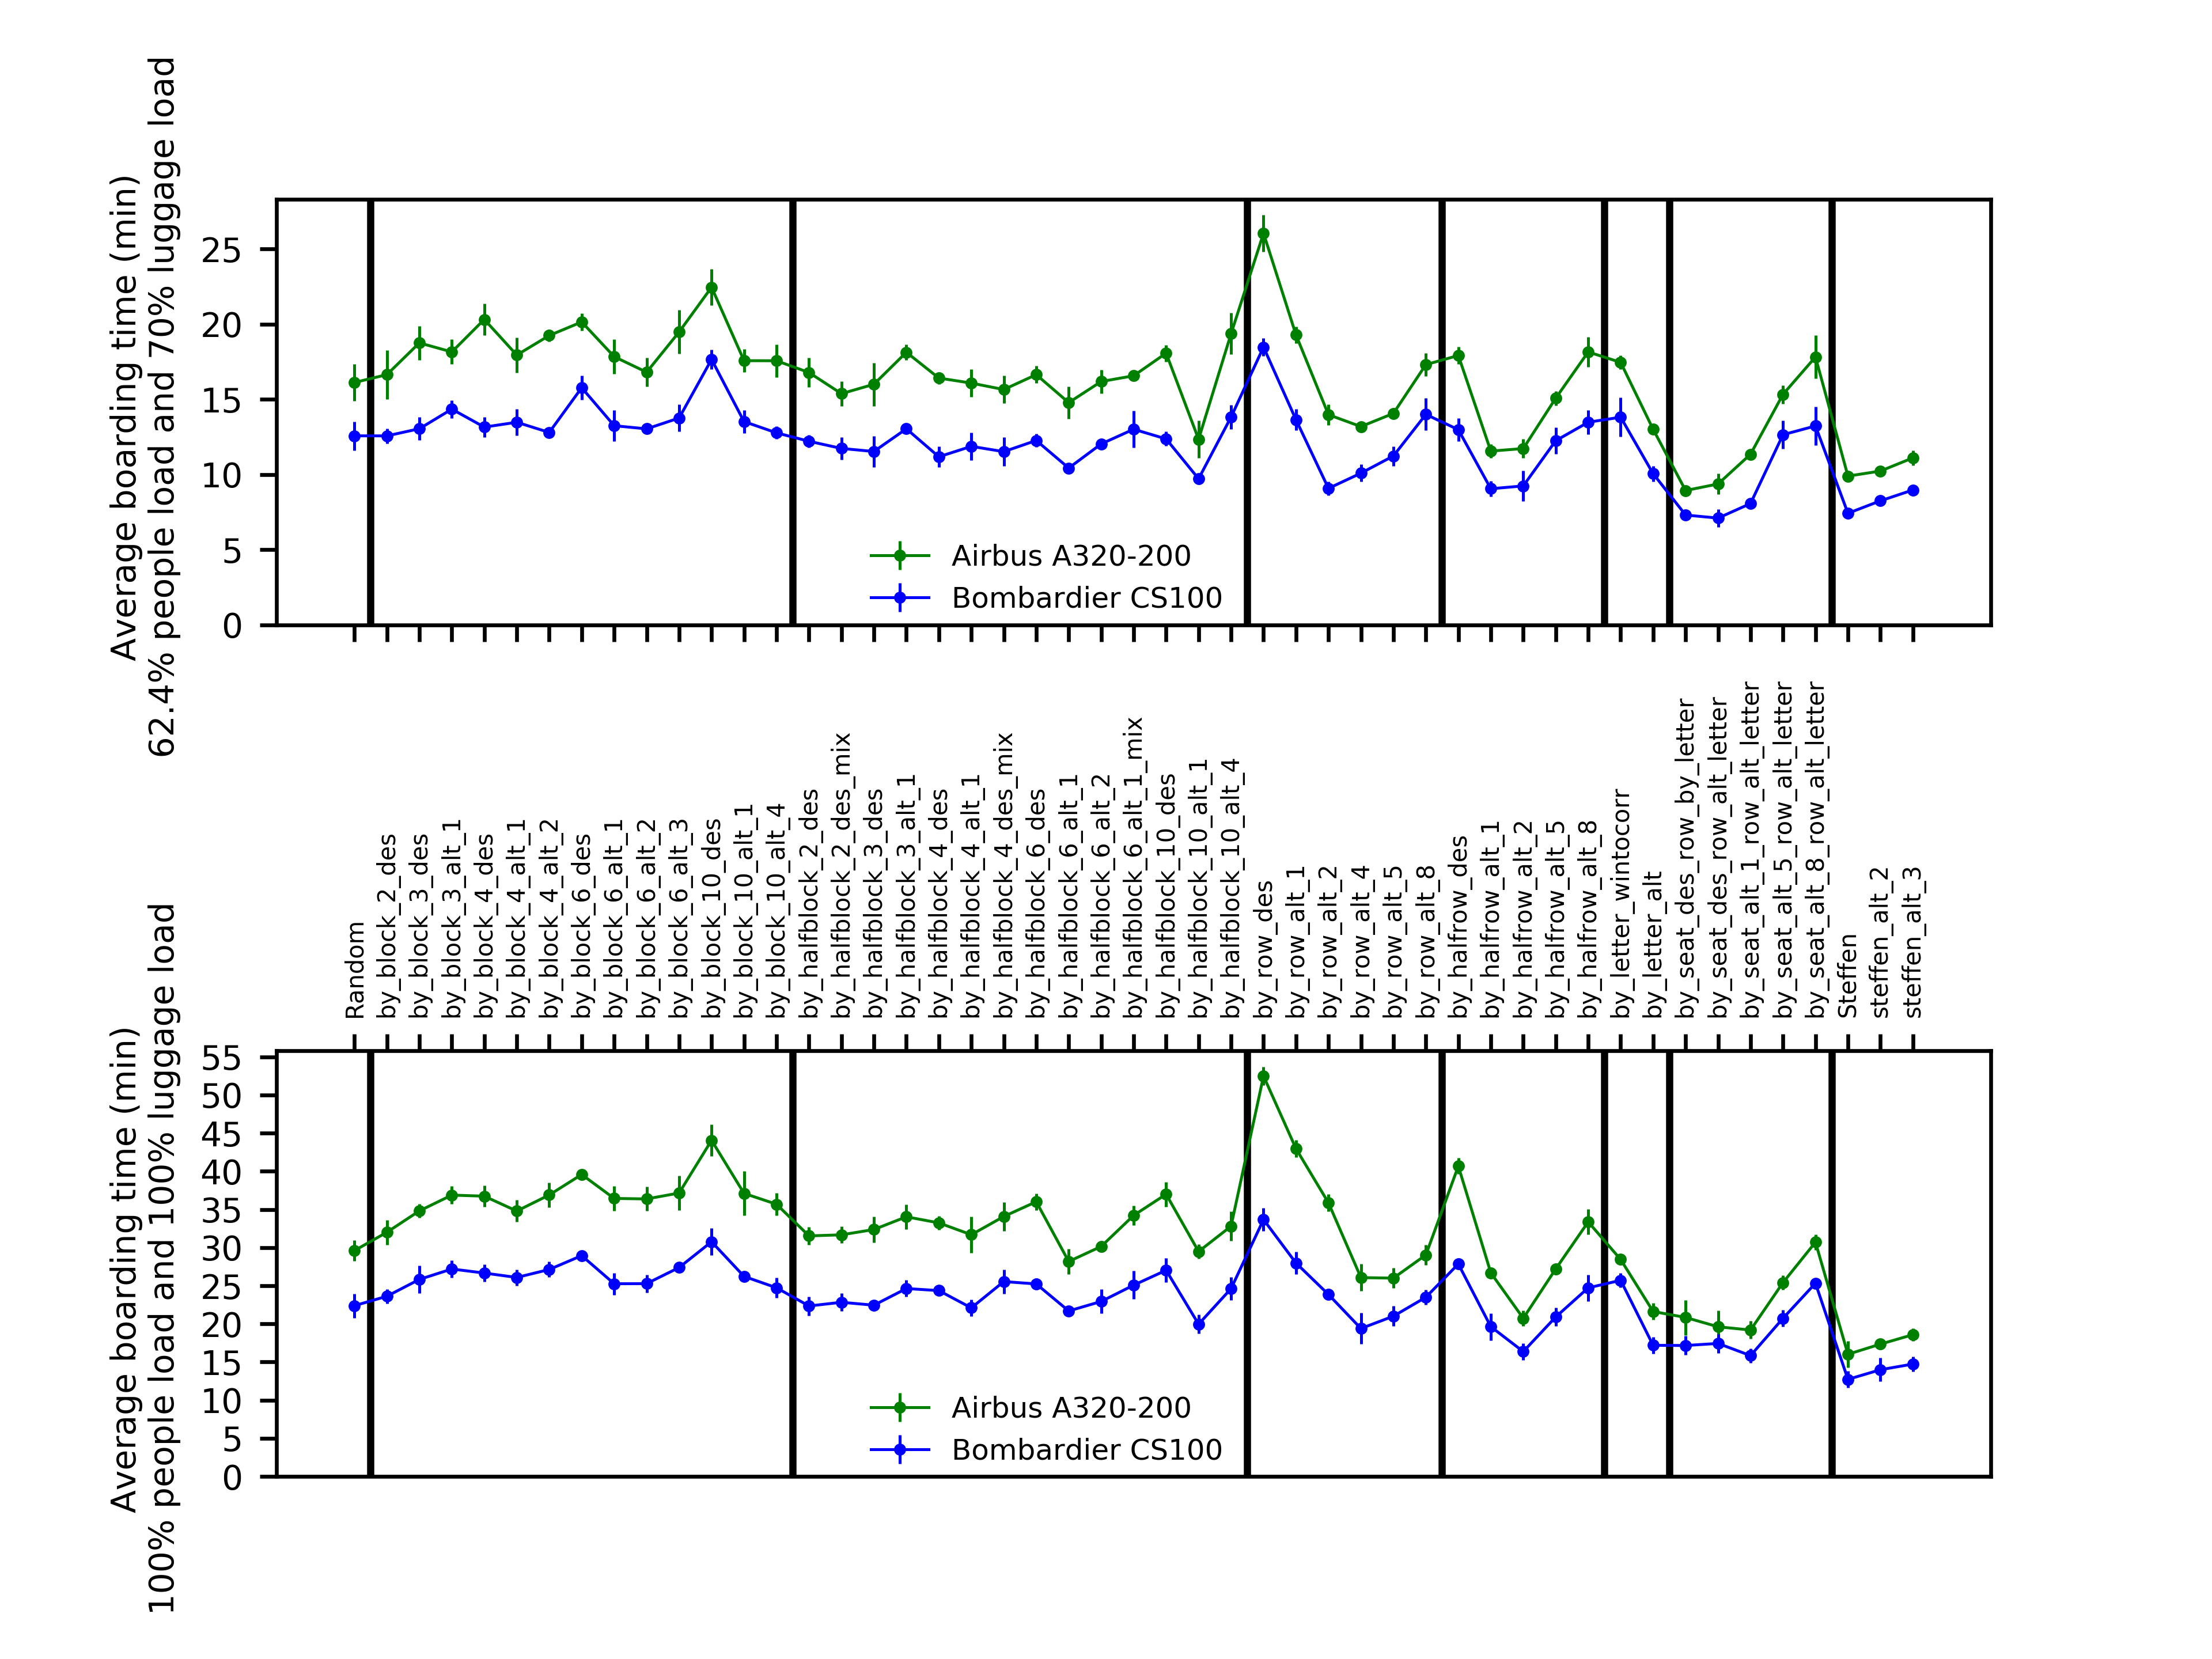
\includegraphics[width=\linewidth]{../../code/AirplaneBoarding/data/figure2/figure2.png}
	\caption{This figure displays the results calculated using our model for the time it takes to board the Bombardier CS100 and the Airbus A320-200 using different boarding methods under a low/high load configuration}
	\label{figure2}
\end{figure}

 
 \subsubsection{Overview}
 In this chapter we compare the results from simulating the 46 boarding methods from \cite{beus} as well as 3 variants of the Steffen method \cite{steffen} on two very modern airplanes, which are currently in the Swiss fleet. For each configuration we again run 5 independent tests and collected the data, which is displayed in Figure \ref{figure2} and stored in table \textit{insert table reference here} (see Appendix). 
 
 
 \paragraph{Airbus A320-200}
 We chose the Airbus A320-200, as it is a commonly used big short-haul plane. Additionally, it has a classical symmetric seat arrangement, so the results we get on the Airbus A320-200 are most likely applicable to many similarly organized planes. 


 \paragraph{Bombardier CS-100}
 The Bombardier CS-100 also is a short-haul plane, but a bit smaller than the Airbus. It is particularly interesting, because its seat are arranged asymetrically, with two seats per row on the left of the aisle, but three per row on the right.  

 \begin{tabular}{l|c c }

	 \hline
	&Airbus A320-200 &Bombardier CS-100 \\
	\hline
\# rows & 30&25   \\
\hline
\# seats right of aisle & 3 & 3 \\
	\hline
	\# seats left of aisle & 3 & 2\\
	\hline
	\# bags per compartment & 5 & 3\\
	\hline
	\\
\end{tabular}

 The most noticeable results are that first of all the Steffen method, which was found in 2008 and has been declared as the potentially fastest boarding method, turns out to perform the best across all test (around 16 minutes for a fully loaded Airbus A320-200) with only a two methods from the ''by\_seat" class coming close (edging out ''Steffen" under not completely full load conditions). Across all 4 configurations, Steffen was around 42\% faster than the most commonly used method, especially on short haul flights, ''Random". Nevertheless ''Random" performed surprisingly well compared to all other methods and is always around the average time across them (this includes methods like Steffen as well). Furthermore, ''Random" performed around 4\% faster than the fastest method from class ''by\_block", who's methods are very common on long haul flights because of larger airplanes with potentially multiple aisles.
 
 
 \subsubsection{Alternation as a key factor}\label{alternation}
 The general trend of the times taken across all boarding methods (in this section we are excluding classes ''Random" and ''by\_letter" because they don't directly deal with rows in any way) reveals an interesting observation. Alternation plays a very key role in the efficiency of methods and can cause significant differences in experienced boarding times. We noticed that for methods, which differentiate themselves from each other only in the alternation, the boarding time first decreases with an increasing alternation and then starts to increase again.
 This effect is more distinct for classes that divide the number of rows in more sections than others, so for example, ''by\_block\_10\_$\dots$", which divides the number of rows into 10 blocks (10 sections), experiences the alternation effect more than ''by\_block\_4\_$\dots$", which only divides the total number of rows into 4 blocks (4 sections)(see Figure \ref{figure2}).  This is also the reason why it is most noticeable for the curves in the sections of method classes ''by\_row" and ''by\_halfrow" in Figure \ref{figure2} because they treat all rows independently from each other, so as separate sections. 
 
 % Maybe add a small paragraph how each boarding method divides there shit into sections
 
 Our explanation for the alternation effect builds upon the observation made by Steffen \cite{steffen} that one of the key factors to boarding efficiency is the number of aisle congestions that occur. As also briefly described in section \ref{model_comp}, congestions caused through luggage storing or actors sitting down arise when actors are unable to move forward because there is another actor in front of them storing their luggage/ sitting down. This usually only happens for actors that have their seats in the same section of the set of sections that the total number of rows were divided into or if the actor waiting has its section further at the back than the actor storing/sitting down (can only happen at the start of the aisle because we always board back to front). Now the reason why, the alternation effect is more distinct for methods, which divide the total number of rows in more sections, is that with fewer sections, the sections increase in size (number of rows included), which means more luggage storing congestions will occur naturally. Therefore, because well chosen alternation parameters can only reduce congestions caused between different sections (not within), alternation effect will increase with a decrease in section size/ increase in number of sections.
 
 The explanation for the decrease and then increase in boarding time with an increasing alternation follows the basic idea of what alternation actually achieves. Alternation decreases the number of row congestions between different sections in the boarding sequence at the expense of space in the aisle. When we start to increase alternation, there will be more space in the aisle between sections that are adjacent in the boarding sequence, so fewer actors will be blocking others from the section that follows next, as they can wait in the new extra space for the congestions within their section to clear up. 
 %TODO CHECK
 This causes the boarding time to decrease as long as the space created is filled with waiting actors. As soon as we start to increase alternation beyond the point where the extra space is effectively used, boarding time will increase again causing the observed effect.
 
  \subsubsection{General observations within each class}
 \paragraph{by\_block}
 For all of the 4 test cases the boarding time appears to be fairly constant compared to the other boarding classes. There are only a few fluctuations, which are caused by the alternation effect. Furthermore, for each test case the best boarding time, which is achieved by the method ''by\_block\_2\_des", is above the average time taken across all tested methods. This indicates that ''by\_block" is not necessarily a class that should be used in practice, for planes similar to ours. 
 \paragraph{by\_halfblock}
 The overall trend of class ''by\_halfblock" is very similar to the one from ''by\_block", but generally a bit lower (so faster). The reason for this is that in this class there is more coordination compared to ''by\_block" because we basically have twice as many blocks to arrange. Generally across all test cases, the best results are achieved with method ''by\_halfblock\_10\_alt\_1". It is interesting to see that the alternation effect behaves is a little different in ''by\_halfblock" compared to ''by\_block", in the later boarding speed increases or remains constant while we increase alternation from 0 to 2 and starts decreasing at 3 (compare methods ''by\_block\_6\_des", ''by\_block\_6\_alt\_1", etc.). In ''by\_halfblock" boarding speed already starts decreasing again, after an initial increase, at alternation 2 (compare methods ''by\_halfblock\_6\_des", ''by\_halfblock\_6\_alt\_1", etc.). This makes sense because, as explained in section \ref{alternation}, increasing alternation will only speed up the boarding process, while the extra aisle space is effectively occupied, but because the sections that the class ''by\_halfblock" creates are only half the size compared to the ones from ''by\_block" (equivalent methods in terms of number of blocks), the increase in boarding speed will reach its maximum earlier. 
 \paragraph{by\_row}
 This class really displays the alternation effect because the methods within it treat each whole row as its own section and only apply different alternations to the order. The method ''by\_row\_des" has the worst boarding time from all methods across all test cases. Its maximum time is almost 52.5 minutes for the fully loaded Airbus A320-200, which is almost twice the average for that configuration. This seems a bit extreme, but considering the fact that everyone will be waiting for the first person to take their seat, then the second etc., before they are able to move forward, it does not really surprise us that it performs the worst. For the Airbus A320-200, the fastest method in this class is the ''by\_row\_alt\_4", which cuts the time taken down to a little less than 26.1 minutes (less than half the maximum) just by perfectly utilizing the Alternation effect. Any further increase in alternation causes the boarding speed to slow down, as expected from our analysis
 
 \paragraph{by\_halfrow}
 ''by\_halfrow" displays the very similar trend compared to ''by\_row" as ''by\_halfblock" did to ''by\_block" in terms of the alternation effect and overall boarding times, which is why I won't go into anymore detail about it. For explicit numbers please have a look at the Appendix. 
 
 \paragraph{by\_letter}
 The two methods that were tested from this class clearly represent the results that we expected because the method ''by\_letter\_wintocorr" fills the seat-columns from left to right, so each actor that has a window seat on the right site will have to wait for two other actors (in our two planes there are 3 seats on the right side) that are already seated in his row to get up and let him in. This is not the case for the second method ''by\_letter\_alt", as it boards the seat-columns from both window seats towards the aisle, which explains why it is significantly faster.
 
 \paragraph{by\_seat}
 The trend for this class depends on the load condition. For the full load, we again experience the alternation effect, with an initial slight decrease in boarding time and then an increase, and already explained in section \ref{model_comp} why they take longer than the first row alternating sequence. Under 62.5\% people and 70\% luggage load we only observe an increase in the boarding time and not the regular pattern. The most likely reason for this is that because we assign a specific order according to seats and the plane is not completely full, not a lot of row congestions happen naturally anymore. Furthermore, under full load alternating already only slightly improved the boarding time, which would explain why it does not have any further positive impact under reduced load. 
 
 \paragraph{Steffen}
 Now, as mentioned in the overview, the original Steffen generally performed the best across all tests. The way Steffen's method achieves this is that it tries to keep the aisle as full as possible, by using a small alternation just big enough to avoid congestions caused through storing or sitting down, in addition to boarding from the windows towards the aisle. Further increasing the alternation did not improve the boarding times, probably because the effect of alternation was already maxed out. Under full load it performed the best across all 49 methods, but under reduced load the first two methods of the ''by\_seat" class just edged it out, most likely because of the same argument as given in ''by\_seat", for why alternation did not improve the result any more, as Steffen uses some alternation. 
 
 
 
 \subsubsection{Effect of plane type and load configuration}
 \paragraph{Effect of load configuration}
 We have seen in the analysis of the ''by\_seat" class in the previous section that the load configuration has an influence on the extend, to which the alternation effect has an impact on boarding methods. So for a reduced load level, as the one used for the data to the first subplot of Figure \ref{figure2}, the alternation effect is only partly influential on very coordinated boarding methods, an increased alternation might only have a negative effect. Under full load we saw that generally all boarding methods took longer than under reduced load. Furthermore, ''Steffen" was the best method as predicted, which is why we assume that the higher the load configuration the more important the choice of boarding method becomes.
 
 \paragraph{Effect of plane type}
 The plane type impacts the boarding time depending on its size, so generally the larger the more seats a plane has, the longer any boarding method will take. Additionally, it was interesting to see that when the plane is asymmetric like the Bombarider CS100 it does not significantly affect the relationships between different boarding methods.
 
 \subsection{Individual Boarding Times - Bombardier CS100 \& Airbus A320-200}
	\begin{figure}
		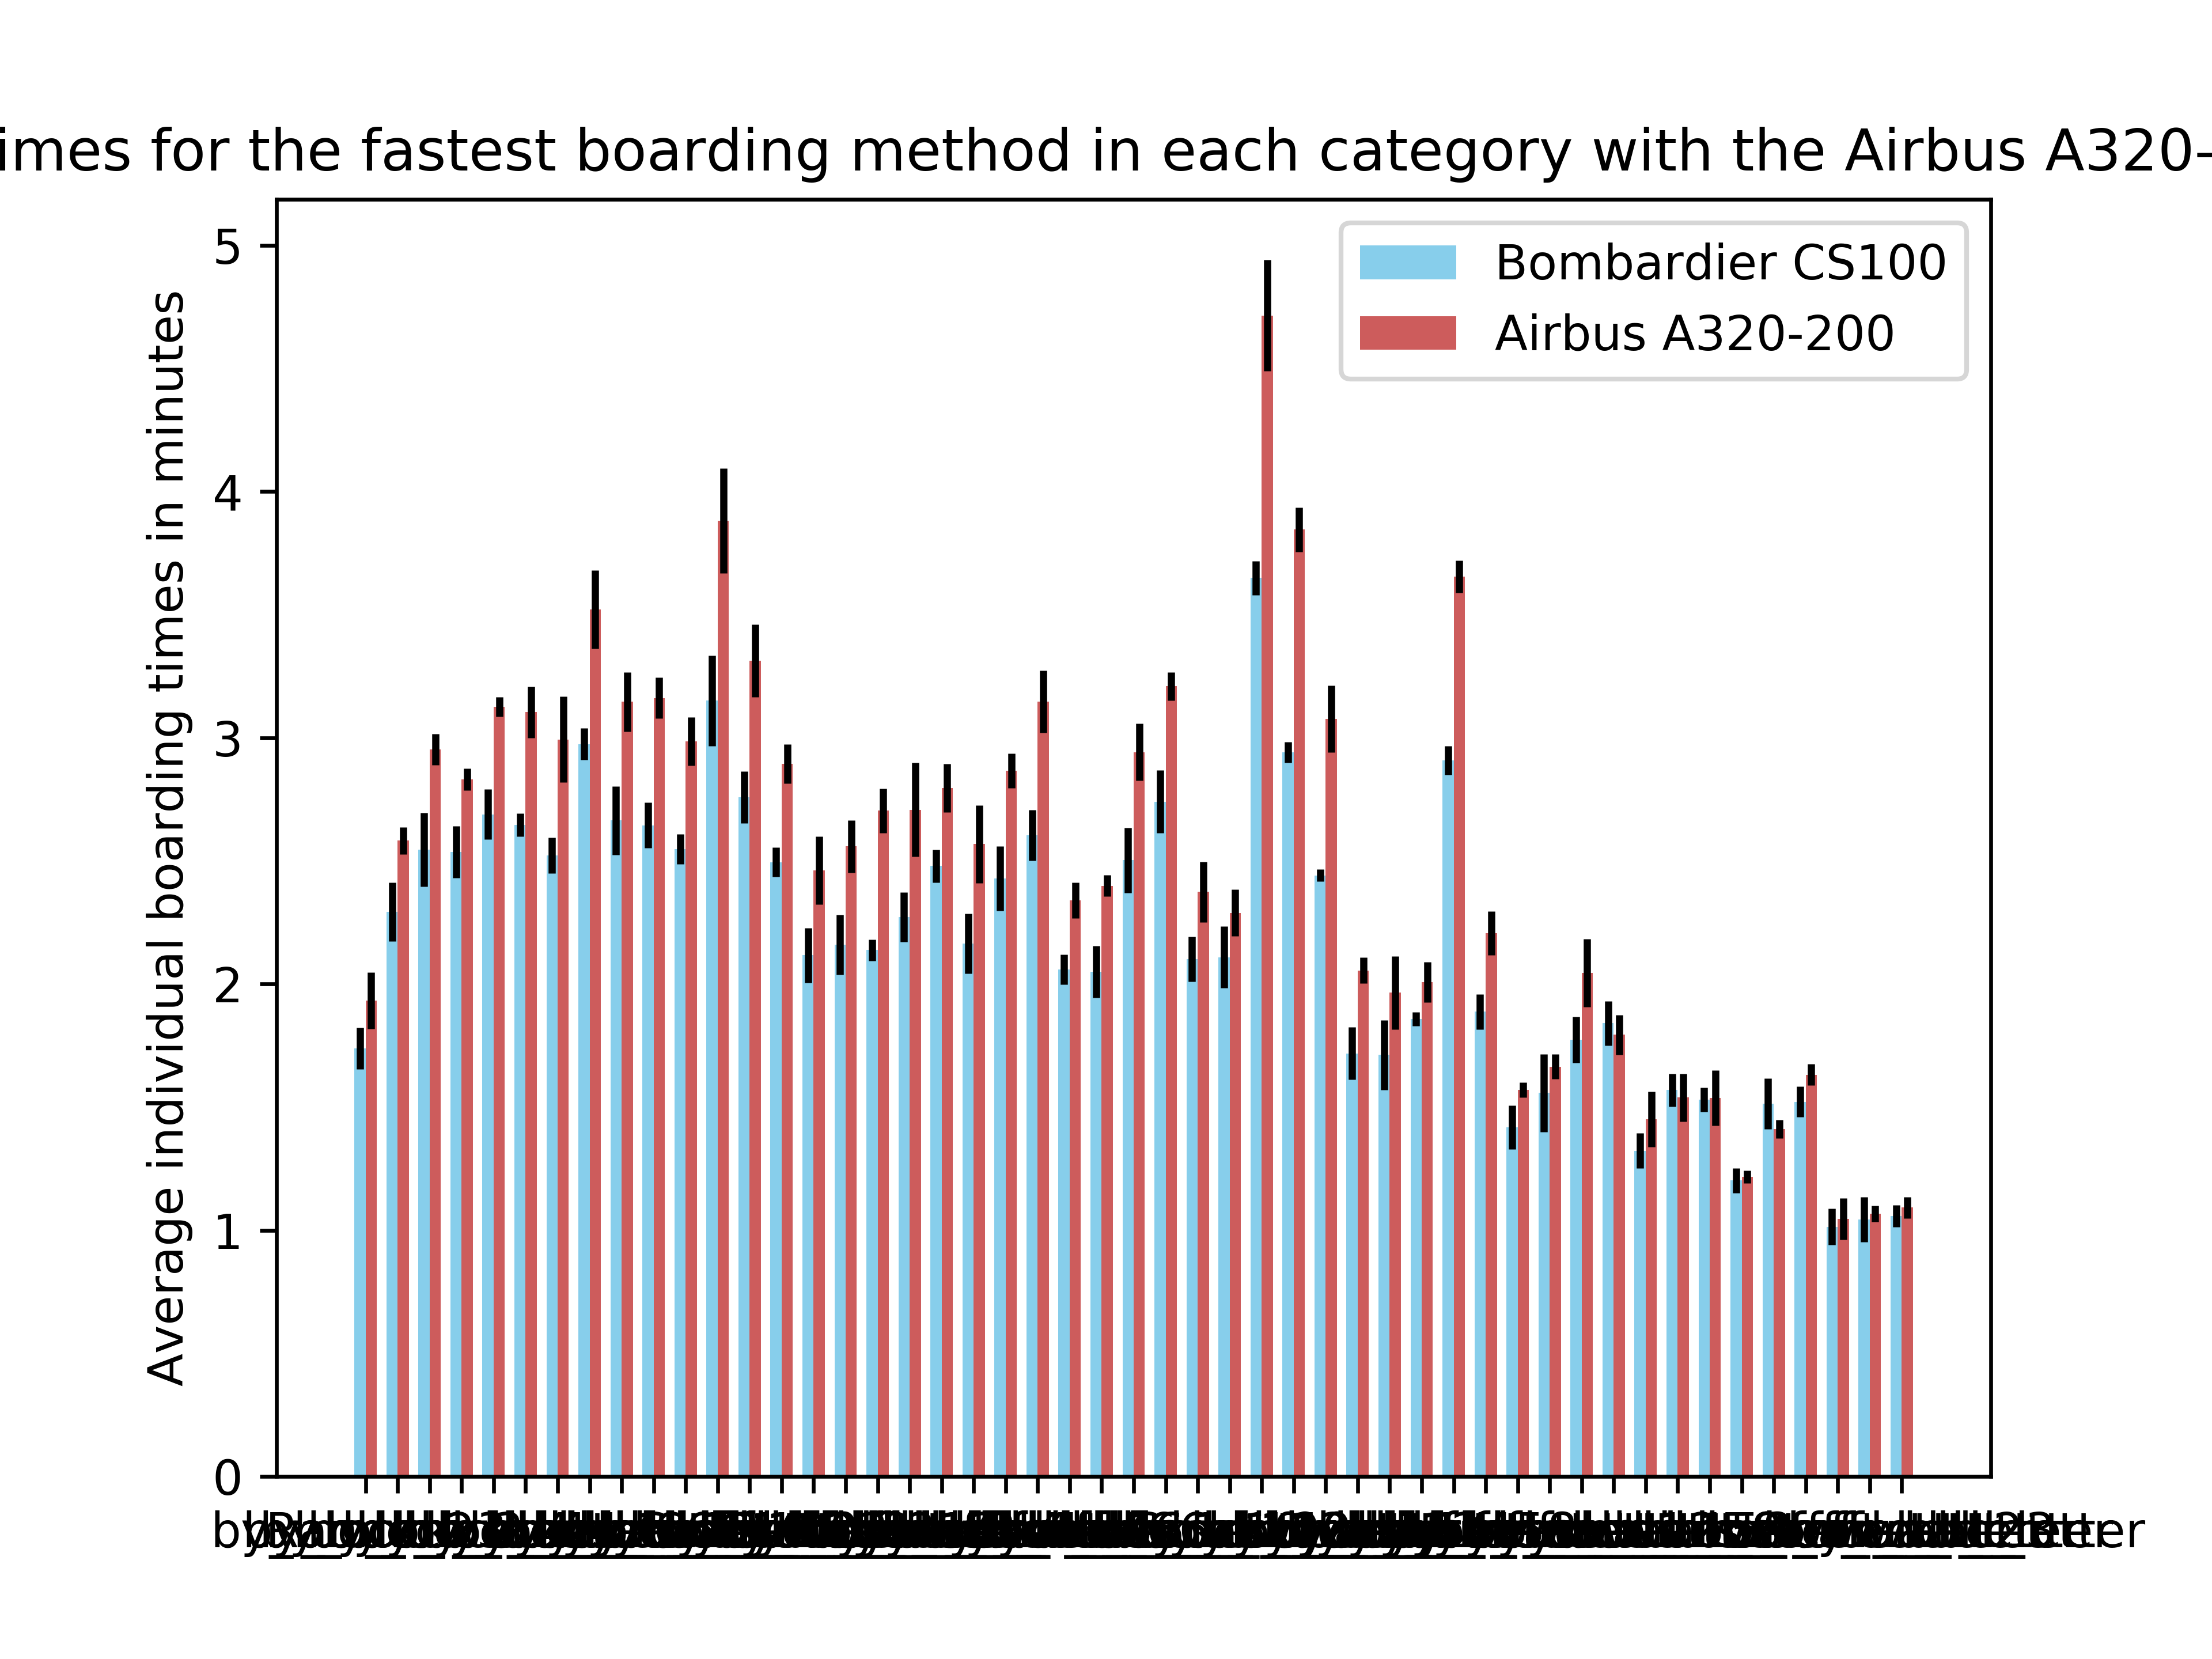
\includegraphics[width=\linewidth]{../../code/AirplaneBoarding/data/figure3/figure3.png}
		\caption{This figure displays the results calculated by our model for the average time it takes each passenger to board the Bombardier CS100 and the Airbus A320-200 using different boarding methods under full load (passenger and luggage)}
		\label{figure3}
	\end{figure}
	For many airlines the total boarding time is very import, especially for low-budget airlines like Ryanair, however many of the more expensive airlines, like Swiss and Lufthansa, really put a big emphasis on costumer experiences. This is why we also collected the data for the average individual boarding times, for the fastest boarding methods from each class. These can be seen in Figure \ref{figure3}. It is apparent that the faster the boarding method, the lower the average individual boarding time. However despite the Bombardier CS100 having a lot fewer seats than the Airbus A320-200 and a lower boarding time for all its methods under full load, it is recognizable that the faster the method, the closer the individual boarding times for the two planes get. This results in almost exactly the same individual boarding time for the fastest method ''Steffen". The increasing efficiency across the boarding methods might yield this result because due to the decreasing number of congestions, the actors are almost able to walk directly towards their seat in the fastest methods.
	
	In terms of numbers, the fastest method ''Steffen" has an individual boarding time of almost only 1 minute for both planes, whereas the fastest block boarding method has an individual boarding time of around 2.58 minutes for the Airbus and around 2.29 minutes for the Bombardier. So more than two times slower than ''Steffen". From those results, we would believe that there is a strong correlation between total and average individual boarding times, which is true, as the $R^2$ value is greater than 90\%.

\subsection{Impact of carry-on luggage on boarding time for a fully occupied Airbus A320-200}
	\begin{figure}
		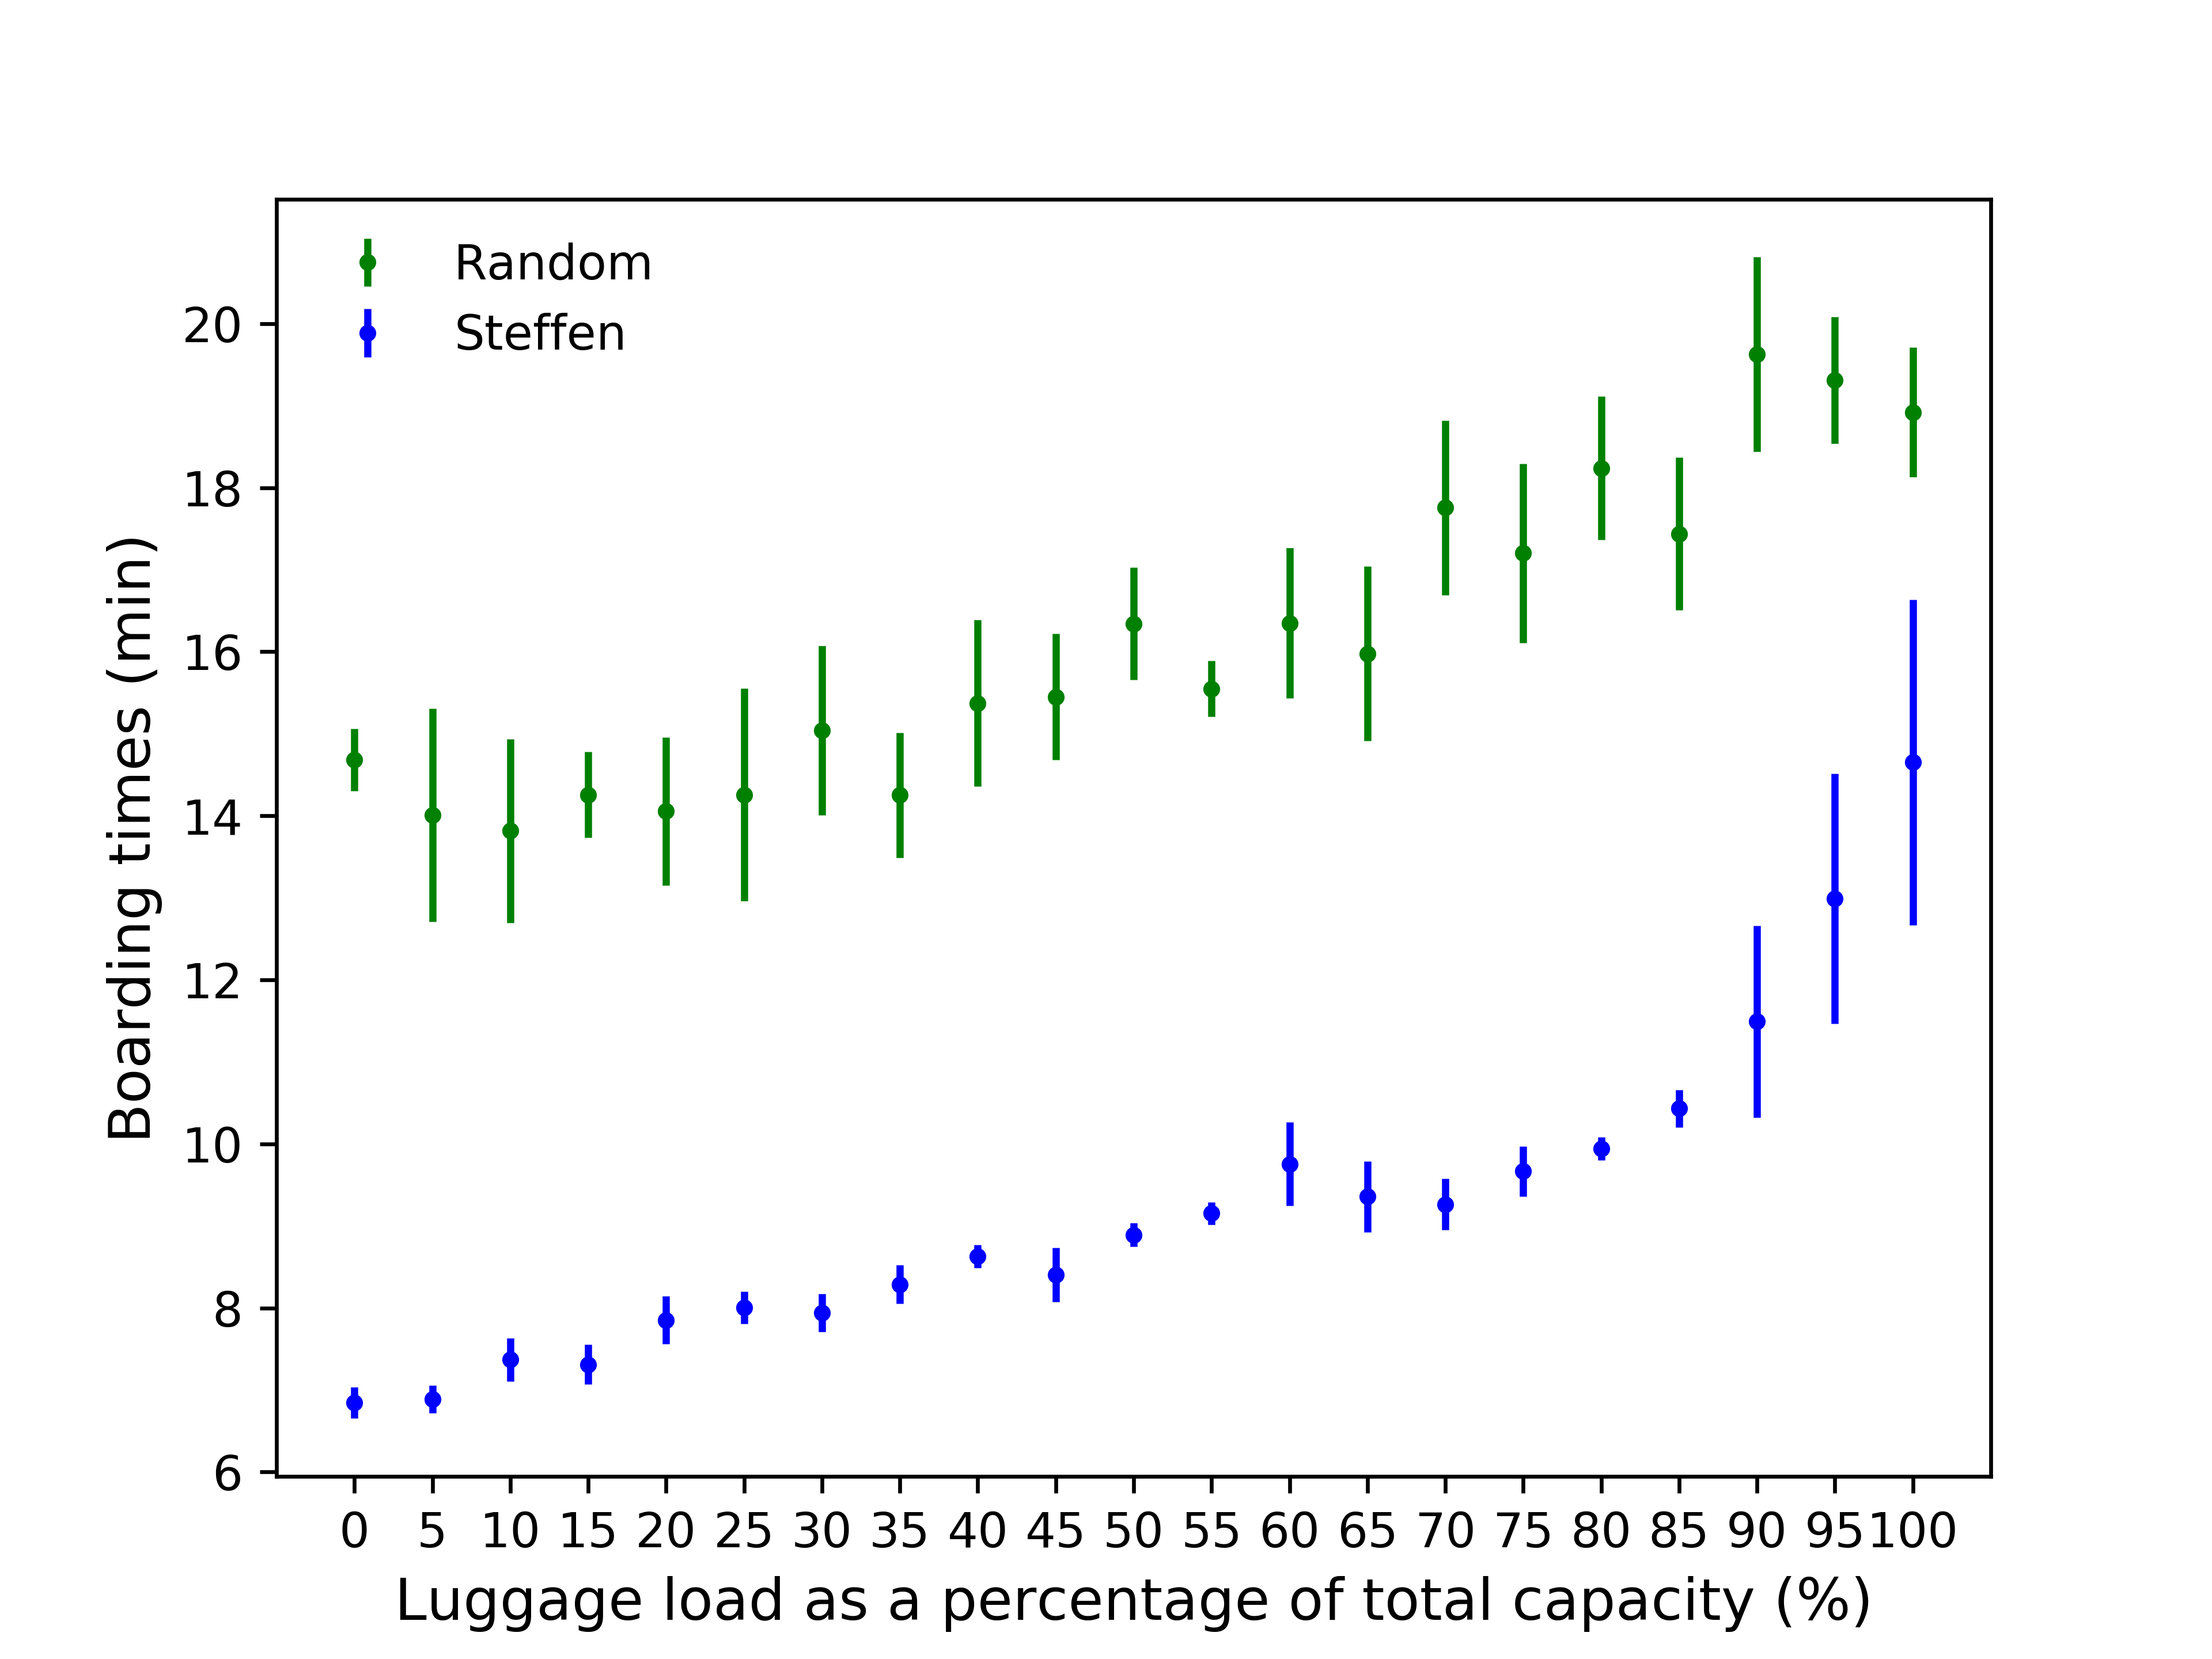
\includegraphics[width=\linewidth]{../../code/AirplaneBoarding/data/figure4/figure4.png}
		\caption{This figure displays the various boarding times with a 95\% confidence interval calculated for the Airbus A320-200 under full passenger load and 21 different luggage load levels using the ''Random" and ''Steffen" method}
		\label{figure4}
	\end{figure}
	\subsubsection{Motivation and relevance}
	We simulated the most commonly used ("Random") and the best boarding method ("Steffen") for different luggage loads, keeping the plane specifications constant (Airbus A320-200) and the passenger load at 100\%, to see what impact carry-on luggage has on the overall boarding time and whether it varies between the two methods. We expect it to be very relevant because it is one major source for row congestions, especially in methods that don't differentiate a lot between different seats (only divide into a small number of sections). This is relevant for many airlines because, for example, there is the option to lower prices for checked-in luggage in order to reduce the amount of carry-on luggage people bring on board, if reducing the boarding time by a significant amount turns out to be more profitable.
	
	\subsubsection{Results and Observations}
	The results from our model can be found in Figure \ref{figure4}. Firstly, they clearly show that our expectation of an upward trend was realistic because ''Steffen" under 100\% luggage load took more than twice as long compared to ''Steffen" under 0\% luggage load. For ''Random" the same comparison amounts to a factor of around 1.3, so luggage seems to have a greater effect on the faster method. Secondly, what also appears is the fact that for ''Steffen", the 95\% confidence area is very small at the beginning but gradually increases with the luggage load (from $\pm 0.218$ minutes up to $\pm 2.26$ minutes). For ''Random" this observation can not be made because the confidence area is always around plus or minus 1 minute ($\pm 10$ seconds) across all measured luggage loads. Lastly, there is a small up and down motion when comparing the different boarding times within each method, while the general upward trend is preserved. This is more noticeable for ''Random" than for ''Steffen". 
	
	\subsubsection{Observation analysis}
		The first observation that luggage has a greater effect on ''Steffen" than on ''Random" can be reduced to the fact that due to the design of Steffen there are generally almost no row congestions caused through people sitting down, which means that the only main source are luggage stores. This is not the case for random boarding because there is no general order specified that would reduce congestions caused through passengers sitting down. 
		
		This also explains the second observation regarding the error bars. Because ''Random" already has no order what so ever specified, an increased luggage load, which is randomly distributed among the actors (described in section \ref{ourmodel}), will most likely not effect introduce any further irregularity. However for ''Steffen", this is a totally different story because there is no indefiniteness within the boarding method, so the more luggage is randomly assigned the more random congestions can possibly occur, which would result in a wider range of measured times.
		
		To conclude, the observed oscillation in the ''Random" method is most likely just a result of the method itself, rather than the luggage, which is why it is not really present in the data of the ''Steffen" method.
	
	

\section{Summary and Outlook}

\subsection{Conclusion}
The comparison between our model and Van Landehems' and Beuselinck's model \cite{beus} showed that the results from our implementation do not differ a lot from theirs and retain the overall trends of the boarding times, as well as relationships between the different boarding methods. This provides good reason to believe that our model accurately depicts reality, as \cite{beus} is generally seen as the foundation for airplane boarding simulations and models. 

Simulating 49 different boarding methods on the two airplanes Airbus A320-200 and Bombardier CS100 revealed some key insights to what the causes of varying boarding times with different boarding methods might be. We found out that the main reason of increased boarding times are congestions in the aisle caused by passengers either storing their luggage or taking their seat because they result in inefficient use of the available space. The boarding methods try to address this issue using different techniques, such as alternation or window to aisle boarding. We found out that one of the major contributing factors in avoiding congestions is the level of alternation that each method employed, as it helps in the attempt to create the perfect balance between the number of passengers that can take their seat or store their luggage concurrently, while not leaving to much free space inside the aisle. However, it can also negative affect boarding time, if not set correctly, which is why careful considerations and evaluations should be made before apply those techniques in practice. Furthermore, we were not only able to observe the high impact that the choice of boarding system has on overall boarding time, but also individual times, which means applying those improved boarding systems in actual airports would allow airlines to not only reduce their turn time, but potentially increase costumer experience. Nevertheless, this would come at the cost of requiring cumbersome procedures at the gates, which most airlines will probably try to avoid. 

\subsection{Limitations}
Our model is an abstract representation of reality, it ignores many aspects such as the increased time it takes to store luggage the fuller the overhead compartments are or personal relationships between passengers. Furthermore, all passengers are represented by uniform actors, which only vary in their moving speeds. Although there is good reason to believe that these factors don't have major impacts on overall boarding times, we believe that the results from our model should only be used to identify the relationships/differences between methods and indication for the overall boarding times, but not exact predictions for the times experienced in practise.

\subsection{Outlook, improvement and extentions}
In order to further improve the model, tests with actual passengers and airplanes should be conducted, as well as further attributes should be added to the actors, in order to be able to differentiate more between different passenger types. Furthermore, we only analysed boarding methods in regards to planes used on short haul flights. It would probably be interesting to find out, to what extend our results hold for larger airplanes like the Airbus A380. 

%TODO final sentance

\section{References}
\begin{thebibliography}{9}
	\bibitem{beus}
	Van Landeghem, H, and A Beuselinck. 
	\textit{"Reducing Passenger Boarding Time in Airplanes: A Simulation Based Approach."} 
	European Journal of Operational Research, vol. 142, no. 2, 2002, pp. 294–308.,
	doi:10.1016/s0377-2217(01)00294-6.
	
	\bibitem{nasa}
	Data Passenger Size from:  NASA. “Man-Systems Integration Standards.” Man-Systems Integration Standards, vol. 1, July 1995, p. 30.
	
	\bibitem{steffen}
	Steffen, Jason H. ''Optimal boarding method for airline passengers." Journal of Air Transport Management 14.3 (2008): 146-150.

\bibitem{barrett} Barrett, Sean D. ''How do the demands for airport services differ between full-service carriers and low-cost carriers?." Journal of air transport management 10.1 (2004): 33-39.


\end{thebibliography}


\section{Appendix}

\begin{table}[htbp]
  \centering
  \caption{Data from our model used for Figure 1}
    \begin{tabular}{rlrrr}
    \multicolumn{1}{l}{No.} &       & \multicolumn{3}{l}{Total Boarding Time (min)} \\
          & Boarding method & \multicolumn{1}{l}{Average} & \multicolumn{1}{l}{S.D.} & \multicolumn{1}{l}{95\% CI} \\
    1     & Random & 2.36E+01 & 1.04E+00 & 1.19E+00 \\
          &       &       &       &  \\
    2     & by\_block\_2\_des & 2.63E+01 & 1.58E+00 & 1.80E+00 \\
    3     & by\_block\_3\_des & 2.68E+01 & 8.86E-01 & 1.01E+00 \\
    4     & by\_block\_3\_alt\_1 & 2.81E+01 & 1.61E+00 & 1.84E+00 \\
    5     & by\_block\_4\_des & 3.07E+01 & 9.24E-01 & 1.05E+00 \\
    6     & by\_block\_4\_alt\_1 & 2.90E+01 & 1.22E+00 & 1.40E+00 \\
    7     & by\_block\_4\_alt\_2 & 2.99E+01 & 1.12E+00 & 1.28E+00 \\
    8     & by\_block\_6\_des & 3.12E+01 & 1.19E+00 & 1.36E+00 \\
    9     & by\_block\_6\_alt\_1 & 3.00E+01 & 1.42E+00 & 1.62E+00 \\
    10    & by\_block\_6\_alt\_2 & 2.94E+01 & 2.43E+00 & 2.77E+00 \\
    11    & by\_block\_6\_alt\_3 & 3.03E+01 & 1.82E+00 & 2.07E+00 \\
    12    & by\_block\_10\_des & 3.49E+01 & 5.90E-01 & 6.73E-01 \\
    13    & by\_block\_10\_alt\_1 & 3.12E+01 & 1.36E+00 & 1.56E+00 \\
    14    & by\_block\_10\_alt\_4 & 2.85E+01 & 1.64E+00 & 1.87E+00 \\
          &       &       &       &  \\
    15    & by\_halfblock\_2\_des & 2.59E+01 & 2.93E+00 & 3.34E+00 \\
    16    & by\_halfblock\_2\_des\_mix & 2.41E+01 & 1.56E+00 & 1.78E+00 \\
    17    & by\_halfblock\_3\_des & 2.48E+01 & 2.05E+00 & 2.34E+00 \\
    18    & by\_halfblock\_3\_alt\_1 & 2.46E+01 & 1.57E+00 & 1.79E+00 \\
    19    & by\_halfblock\_4\_des 2 & 2.61E+01 & 4.14E-01 & 4.72E-01 \\
    20    & by\_halfblock\_4\_alt\_1 & 2.36E+01 & 9.12E-01 & 1.04E+00 \\
    21    & by\_halfblock\_4\_des\_mix & 2.62E+01 & 6.93E-01 & 7.90E-01 \\
    22    & by\_halfblock\_6\_des & 2.82E+01 & 9.75E-01 & 1.11E+00 \\
    23    & by\_halfblock\_6\_alt\_1 & 2.41E+01 & 6.48E-01 & 7.39E-01 \\
    24    & by\_halfblock\_6\_alt\_2 & 2.40E+01 & 7.03E-01 & 8.02E-01 \\
    25    & by\_halfblock\_6\_alt\_1\_mix & 2.35E+01 & 1.93E+00 & 2.21E+00 \\
    26    & by\_halfblock\_10\_des & 2.98E+01 & 1.11E+00 & 1.27E+00 \\
    27    & by\_halfblock\_10\_alt\_1 & 2.43E+01 & 1.14E+00 & 1.30E+00 \\
    28    & by\_halfblock\_10\_alt\_4 & 2.42E+01 & 9.23E-01 & 1.05E+00 \\
          &       &       &       &  \\
    29    & by\_row\_des & 4.20E+01 & 1.26E+00 & 1.44E+00 \\
    30    & by\_row\_alt\_1 & 3.47E+01 & 2.07E+00 & 2.36E+00 \\
    31    & by\_row\_alt\_2 & 2.76E+01 & 6.85E-01 & 7.81E-01 \\
    32    & by\_row\_alt\_4 & 2.16E+01 & 7.04E-01 & 8.04E-01 \\
    33    & by\_row\_alt\_5 & 2.11E+01 & 5.05E-01 & 5.77E-01 \\
    34    & by\_row\_alt\_8 & 2.54E+01 & 7.72E-01 & 8.81E-01 \\
      %    &       &       &       &  \\
    %35    & by\_halfrow\_des & 3.14E+01 & 1.30E+00 & 1.49E+00 \\
    %36    & by\_halfrow\_alt\_1 & 2.09E+01 & 3.87E-01 & 4.41E-01 \\
    %37    & by\_halfrow\_alt\_2 & 1.64E+01 & 1.24E+00 & 1.42E+00 \\
    %38    & by\_halfrow\_alt\_5 & 2.15E+01 & 6.96E-01 & 7.94E-01 \\
    %39    & by\_halfrow\_alt\_8 & 2.67E+01 & 1.31E+00 & 1.50E+00 \\
      %    &       &       &       &  \\
    %40    & by\_letter\_wintocorr & 2.24E+01 & 1.06E+00 & 1.21E+00 \\
    %41    & by\_letter\_alt & 1.57E+01 & 5.39E-01 & 6.14E-01 \\
      %    &       &       &       &  \\
    %42    & by\_seat\_des\_row\_by\_letter & 1.49E+01 & 1.39E+00 & 1.59E+00 \\
    %43    & by\_seat\_des\_row\_alt\_letter & 1.52E+01 & 1.85E+00 & 2.11E+00 \\
    %44    & by\_seat\_alt\_1\_row\_alt\_letter & 1.59E+01 & 1.50E+00 & 1.71E+00 \\
    %45    & by\_seat\_alt\_5\_row\_alt\_letter & 2.12E+01 & 8.83E-01 & 1.01E+00 \\
    %46    & by\_seat\_alt\_8\_row\_alt\_letter & 2.61E+01 & 5.49E-01 & 6.26E-01 \\
    \end{tabular}%

  \label{tab:fig1}%
\end{table}%
\begin{table}[t]
	\centering
	\begin{tabular}{rlrrr}
		 35    & by\_halfrow\_des & 3.14E+01 & 1.30E+00 & 1.49E+00 \\
		36    & by\_halfrow\_alt\_1 & 2.09E+01 & 3.87E-01 & 4.41E-01 \\
		37    & by\_halfrow\_alt\_2 & 1.64E+01 & 1.24E+00 & 1.42E+00 \\
		38    & by\_halfrow\_alt\_5 & 2.15E+01 & 6.96E-01 & 7.94E-01 \\
		39    & by\_halfrow\_alt\_8 & 2.67E+01 & 1.31E+00 & 1.50E+00 \\
		&       &       &       &  \\
		40    & by\_letter\_wintocorr & 2.24E+01 & 1.06E+00 & 1.21E+00 \\
		41    & by\_letter\_alt & 1.57E+01 & 5.39E-01 & 6.14E-01 \\
		&       &       &       &  \\
		42    & by\_seat\_des\_row\_by\_letter & 1.49E+01 & 1.39E+00 & 1.59E+00 \\
		43    & by\_seat\_des\_row\_alt\_letter & 1.52E+01 & 1.85E+00 & 2.11E+00 \\
		44    & by\_seat\_alt\_1\_row\_alt\_letter & 1.59E+01 & 1.50E+00 & 1.71E+00 \\
		45    & by\_seat\_alt\_5\_row\_alt\_letter & 2.12E+01 & 8.83E-01 & 1.01E+00 \\
		46    & by\_seat\_alt\_8\_row\_alt\_letter & 2.61E+01 & 5.49E-01 & 6.26E-01 \\
	\end{tabular}
\end{table}
% Table generated by Excel2LaTeX from sheet 'Sheet1'
\begin{table}[htbp]
  \centering
  \caption{Add caption}
    \begin{tabular}{rlrrrrrrrrrrrr}
    \multicolumn{1}{l}{No.} &       & \multicolumn{3}{l}{Bombadier CS100 full load} & \multicolumn{3}{l}{Bombadier CS100 normal load} & \multicolumn{3}{l}{Airbus A320-200 full load} & \multicolumn{3}{l}{Airbus A320-200 normal load} \\
          &       & \multicolumn{3}{l}{Total Boarding Time (min)} & \multicolumn{3}{l}{Total Boarding Time (min)} & \multicolumn{3}{l}{Total Boarding Time (min)} & \multicolumn{3}{l}{Total Boarding Time (min)} \\
          & Boarding method & \multicolumn{1}{l}{Average} & \multicolumn{1}{l}{S.D.} & \multicolumn{1}{l}{95\% CI} & \multicolumn{1}{l}{Average} & \multicolumn{1}{l}{S.D.} & \multicolumn{1}{l}{95\% CI} & \multicolumn{1}{l}{Average} & \multicolumn{1}{l}{S.D.} & \multicolumn{1}{l}{95\% CI} & \multicolumn{1}{l}{Average} & \multicolumn{1}{l}{S.D.} & \multicolumn{1}{l}{95\% CI} \\
    1     & Random & 2.24E+01 & 1.57E+00 & 1.79E+00 & 1.26E+01 & 9.61E-01 & 1.10E+00 & 2.96E+01 & 1.37E+00 & 1.56E+00 & 1.61E+01 & 1.24E+00 & 1.42E+00 \\
          &       &       &       &       &       &       &       &       &       &       &       &       &  \\
    2     & by\_block\_2\_des & 2.36E+01 & 9.64E-01 & 1.10E+00 & 1.26E+01 & 4.93E-01 & 5.63E-01 & 3.20E+01 & 1.63E+00 & 1.86E+00 & 1.66E+01 & 1.64E+00 & 1.87E+00 \\
    3     & by\_block\_3\_des & 2.58E+01 & 1.84E+00 & 2.10E+00 & 1.30E+01 & 7.67E-01 & 8.75E-01 & 3.48E+01 & 9.32E-01 & 1.06E+00 & 1.88E+01 & 1.12E+00 & 1.28E+00 \\
    4     & by\_block\_3\_alt\_1 & 2.72E+01 & 1.14E+00 & 1.31E+00 & 1.44E+01 & 5.98E-01 & 6.82E-01 & 3.69E+01 & 1.18E+00 & 1.35E+00 & 1.82E+01 & 8.24E-01 & 9.41E-01 \\
    5     & by\_block\_4\_des & 2.67E+01 & 1.14E+00 & 1.30E+00 & 1.32E+01 & 6.77E-01 & 7.73E-01 & 3.67E+01 & 1.37E+00 & 1.56E+00 & 2.03E+01 & 1.07E+00 & 1.22E+00 \\
    6     & by\_block\_4\_alt\_1 & 2.61E+01 & 1.05E+00 & 1.20E+00 & 1.35E+01 & 8.93E-01 & 1.02E+00 & 3.48E+01 & 1.43E+00 & 1.63E+00 & 1.79E+01 & 1.17E+00 & 1.33E+00 \\
    7     & by\_block\_4\_alt\_2 & 2.71E+01 & 1.03E+00 & 1.17E+00 & 1.28E+01 & 2.97E-01 & 3.39E-01 & 3.69E+01 & 1.65E+00 & 1.89E+00 & 1.92E+01 & 4.07E-01 & 4.65E-01 \\
    8     & by\_block\_6\_des & 2.89E+01 & 6.54E-01 & 7.46E-01 & 1.58E+01 & 7.89E-01 & 9.00E-01 & 3.96E+01 & 6.59E-01 & 7.51E-01 & 2.01E+01 & 5.78E-01 & 6.59E-01 \\
    9     & by\_block\_6\_alt\_1 & 2.53E+01 & 1.44E+00 & 1.64E+00 & 1.32E+01 & 1.02E+00 & 1.16E+00 & 3.64E+01 & 1.63E+00 & 1.86E+00 & 1.78E+01 & 1.15E+00 & 1.31E+00 \\
    10    & by\_block\_6\_alt\_2 & 2.53E+01 & 1.15E+00 & 1.31E+00 & 1.30E+01 & 2.55E-01 & 2.90E-01 & 3.64E+01 & 1.59E+00 & 1.81E+00 & 1.68E+01 & 9.57E-01 & 1.09E+00 \\
    11    & by\_block\_6\_alt\_3 & 2.74E+01 & 2.05E-01 & 2.33E-01 & 1.38E+01 & 9.01E-01 & 1.03E+00 & 3.71E+01 & 2.28E+00 & 2.60E+00 & 1.95E+01 & 1.45E+00 & 1.66E+00 \\
    12    & by\_block\_10\_des & 3.08E+01 & 1.76E+00 & 2.01E+00 & 1.77E+01 & 6.43E-01 & 7.33E-01 & 4.41E+01 & 2.09E+00 & 2.39E+00 & 2.25E+01 & 1.22E+00 & 1.39E+00 \\
    13    & by\_block\_10\_alt\_1 & 2.62E+01 & 5.73E-01 & 6.54E-01 & 1.35E+01 & 7.77E-01 & 8.86E-01 & 3.71E+01 & 2.89E+00 & 3.30E+00 & 1.76E+01 & 7.54E-01 & 8.60E-01 \\
    14    & by\_block\_10\_alt\_4 & 2.47E+01 & 1.35E+00 & 1.54E+00 & 1.28E+01 & 4.22E-01 & 4.81E-01 & 3.57E+01 & 1.48E+00 & 1.68E+00 & 1.76E+01 & 1.10E+00 & 1.26E+00 \\
          &       &       &       &       &       &       &       &       &       &       &       &       &  \\
    15    & by\_halfblock\_2\_des & 2.23E+01 & 1.25E+00 & 1.43E+00 & 1.22E+01 & 4.23E-01 & 4.83E-01 & 3.15E+01 & 1.17E+00 & 1.34E+00 & 1.68E+01 & 9.68E-01 & 1.10E+00 \\
    16    & by\_halfblock\_2\_des\_mix & 2.28E+01 & 1.18E+00 & 1.35E+00 & 1.17E+01 & 7.34E-01 & 8.37E-01 & 3.17E+01 & 1.08E+00 & 1.24E+00 & 1.54E+01 & 8.32E-01 & 9.50E-01 \\
    17    & by\_halfblock\_3\_des & 2.25E+01 & 4.59E-01 & 5.24E-01 & 1.15E+01 & 1.03E+00 & 1.18E+00 & 3.24E+01 & 1.71E+00 & 1.95E+00 & 1.60E+01 & 1.44E+00 & 1.64E+00 \\
    18    & by\_halfblock\_3\_alt\_1 & 2.46E+01 & 1.09E+00 & 1.24E+00 & 1.30E+01 & 3.25E-01 & 3.71E-01 & 3.40E+01 & 1.64E+00 & 1.87E+00 & 1.81E+01 & 5.32E-01 & 6.07E-01 \\
    19    & by\_halfblock\_4\_des 2 & 2.44E+01 & 5.44E-01 & 6.20E-01 & 1.12E+01 & 6.92E-01 & 7.89E-01 & 3.32E+01 & 9.23E-01 & 1.05E+00 & 1.64E+01 & 4.12E-01 & 4.70E-01 \\
    20    & by\_halfblock\_4\_alt\_1 & 2.21E+01 & 1.12E+00 & 1.28E+00 & 1.19E+01 & 9.07E-01 & 1.03E+00 & 3.17E+01 & 2.35E+00 & 2.68E+00 & 1.61E+01 & 9.13E-01 & 1.04E+00 \\
    21    & by\_halfblock\_4\_des\_mix & 2.55E+01 & 1.58E+00 & 1.80E+00 & 1.15E+01 & 9.54E-01 & 1.09E+00 & 3.41E+01 & 1.86E+00 & 2.13E+00 & 1.57E+01 & 9.15E-01 & 1.04E+00 \\
    22    & by\_halfblock\_6\_des & 2.52E+01 & 7.56E-01 & 8.63E-01 & 1.23E+01 & 4.53E-01 & 5.17E-01 & 3.60E+01 & 1.09E+00 & 1.24E+00 & 1.66E+01 & 5.77E-01 & 6.58E-01 \\
    23    & by\_halfblock\_6\_alt\_1 & 2.17E+01 & 5.64E-01 & 6.43E-01 & 1.04E+01 & 3.37E-01 & 3.84E-01 & 2.82E+01 & 1.67E+00 & 1.91E+00 & 1.48E+01 & 1.06E+00 & 1.20E+00 \\
    24    & by\_halfblock\_6\_alt\_2 & 2.29E+01 & 1.57E+00 & 1.80E+00 & 1.20E+01 & 3.18E-01 & 3.63E-01 & 3.01E+01 & 6.29E-01 & 7.17E-01 & 1.62E+01 & 7.92E-01 & 9.03E-01 \\
    25    & by\_halfblock\_6\_alt\_1\_mix & 2.51E+01 & 1.85E+00 & 2.11E+00 & 1.30E+01 & 1.23E+00 & 1.40E+00 & 3.42E+01 & 1.27E+00 & 1.45E+00 & 1.66E+01 & 2.81E-01 & 3.20E-01 \\
    26    & by\_halfblock\_10\_des & 2.70E+01 & 1.57E+00 & 1.80E+00 & 1.24E+01 & 4.80E-01 & 5.48E-01 & 3.70E+01 & 1.61E+00 & 1.84E+00 & 1.81E+01 & 5.57E-01 & 6.36E-01 \\
    27    & by\_halfblock\_10\_alt\_1 & 2.00E+01 & 1.23E+00 & 1.40E+00 & 9.72E+00 & 3.68E-01 & 4.20E-01 & 2.95E+01 & 9.47E-01 & 1.08E+00 & 1.23E+01 & 1.26E+00 & 1.43E+00 \\
    28    & by\_halfblock\_10\_alt\_4 & 2.46E+01 & 1.50E+00 & 1.72E+00 & 1.38E+01 & 8.04E-01 & 9.17E-01 & 3.28E+01 & 1.94E+00 & 2.21E+00 & 1.94E+01 & 1.38E+00 & 1.57E+00 \\
          &       &       &       &       &       &       &       &       &       &       &       &       &  \\
    29    & by\_row\_des & 3.37E+01 & 1.51E+00 & 1.73E+00 & 1.85E+01 & 5.90E-01 & 6.73E-01 & 5.25E+01 & 1.22E+00 & 1.39E+00 & 2.60E+01 & 1.23E+00 & 1.41E+00 \\
    30    & by\_row\_alt\_1 & 2.80E+01 & 1.46E+00 & 1.66E+00 & 1.36E+01 & 6.98E-01 & 7.96E-01 & 4.30E+01 & 1.13E+00 & 1.29E+00 & 1.93E+01 & 5.70E-01 & 6.50E-01 \\
    31    & by\_row\_alt\_2 & 2.39E+01 & 7.38E-01 & 8.42E-01 & 9.08E+00 & 4.58E-01 & 5.22E-01 & 3.59E+01 & 1.11E+00 & 1.26E+00 & 1.40E+01 & 6.96E-01 & 7.93E-01 \\
    32    & by\_row\_alt\_4 & 1.94E+01 & 2.03E+00 & 2.32E+00 & 1.01E+01 & 5.75E-01 & 6.56E-01 & 2.61E+01 & 1.78E+00 & 2.03E+00 & 1.32E+01 & 2.77E-01 & 3.16E-01 \\
    33    & by\_row\_alt\_5 & 2.10E+01 & 1.32E+00 & 1.51E+00 & 1.12E+01 & 6.54E-01 & 7.46E-01 & 2.60E+01 & 1.33E+00 & 1.52E+00 & 1.41E+01 & 3.29E-01 & 3.76E-01 \\
    34    & by\_row\_alt\_8 & 2.35E+01 & 9.82E-01 & 1.12E+00 & 1.40E+01 & 1.07E+00 & 1.22E+00 & 2.90E+01 & 1.35E+00 & 1.54E+00 & 1.73E+01 & 7.65E-01 & 8.73E-01 \\
          &       &       &       &       &       &       &       &       &       &       &       &       &  \\
    35    & by\_halfrow\_des & 2.79E+01 & 4.53E-01 & 5.17E-01 & 1.30E+01 & 7.75E-01 & 8.84E-01 & 4.07E+01 & 1.06E+00 & 1.21E+00 & 1.79E+01 & 5.80E-01 & 6.62E-01 \\
    36    & by\_halfrow\_alt\_1 & 1.96E+01 & 1.78E+00 & 2.03E+00 & 9.06E+00 & 5.32E-01 & 6.07E-01 & 2.67E+01 & 7.60E-01 & 8.67E-01 & 1.16E+01 & 4.61E-01 & 5.26E-01 \\
    37    & by\_halfrow\_alt\_2 & 1.64E+01 & 1.10E+00 & 1.25E+00 & 9.24E+00 & 1.00E+00 & 1.14E+00 & 2.07E+01 & 1.04E+00 & 1.19E+00 & 1.17E+01 & 6.27E-01 & 7.15E-01 \\
    38    & by\_halfrow\_alt\_5 & 2.09E+01 & 1.21E+00 & 1.38E+00 & 1.23E+01 & 8.69E-01 & 9.91E-01 & 2.72E+01 & 7.33E-01 & 8.36E-01 & 1.51E+01 & 4.76E-01 & 5.43E-01 \\
    39    & by\_halfrow\_alt\_8 & 2.47E+01 & 1.75E+00 & 1.99E+00 & 1.35E+01 & 7.87E-01 & 8.98E-01 & 3.34E+01 & 1.65E+00 & 1.88E+00 & 1.82E+01 & 9.98E-01 & 1.14E+00 \\
          &       &       &       &       &       &       &       &       &       &       &       &       &  \\
    40    & by\_letter\_wintocorr & 2.57E+01 & 9.41E-01 & 1.07E+00 & 1.38E+01 & 1.31E+00 & 1.49E+00 & 2.84E+01 & 7.26E-01 & 8.28E-01 & 1.75E+01 & 4.55E-01 & 5.19E-01 \\
    41    & by\_letter\_alt & 1.72E+01 & 1.12E+00 & 1.28E+00 & 1.01E+01 & 5.21E-01 & 5.94E-01 & 2.16E+01 & 1.10E+00 & 1.26E+00 & 1.30E+01 & 2.31E-01 & 2.63E-01 \\
          &       &       &       &       &       &       &       &       &       &       &       &       &  \\
    42    & by\_seat\_des\_row\_by\_letter & 1.72E+01 & 1.24E+00 & 1.41E+00 & 7.31E+00 & 6.20E-02 & 7.08E-02 & 2.08E+01 & 2.30E+00 & 2.62E+00 & 8.94E+00 & 2.52E-01 & 2.87E-01 \\
    43    & by\_seat\_des\_row\_alt\_letter & 1.74E+01 & 1.25E+00 & 1.42E+00 & 7.10E+00 & 5.82E-01 & 6.64E-01 & 1.96E+01 & 2.13E+00 & 2.43E+00 & 9.37E+00 & 6.86E-01 & 7.83E-01 \\
    44    & by\_seat\_alt\_1\_row\_alt\_letter & 1.58E+01 & 9.49E-01 & 1.08E+00 & 8.07E+00 & 3.36E-01 & 3.84E-01 & 1.92E+01 & 1.17E+00 & 1.33E+00 & 1.14E+01 & 3.39E-01 & 3.87E-01 \\
    45    & by\_seat\_alt\_5\_row\_alt\_letter & 2.07E+01 & 1.13E+00 & 1.29E+00 & 1.27E+01 & 9.32E-01 & 1.06E+00 & 2.54E+01 & 9.43E-01 & 1.08E+00 & 1.53E+01 & 6.12E-01 & 6.98E-01 \\
    46    & by\_seat\_alt\_8\_row\_alt\_letter & 2.53E+01 & 5.28E-01 & 6.02E-01 & 1.32E+01 & 1.30E+00 & 1.48E+00 & 3.07E+01 & 1.04E+00 & 1.19E+00 & 1.78E+01 & 1.44E+00 & 1.64E+00 \\
          &       &       &       &       &       &       &       &       &       &       &       &       &  \\
    47    & Steffen & 1.27E+01 & 1.07E+00 & 1.22E+00 & 7.42E+00 & 3.51E-01 & 4.00E-01 & 1.60E+01 & 1.70E+00 & 1.94E+00 & 9.90E+00 & 2.64E-01 & 3.01E-01 \\
    48    & steffen\_alt\_2 & 1.40E+01 & 1.54E+00 & 1.75E+00 & 8.25E+00 & 2.53E-01 & 2.88E-01 & 1.73E+01 & 3.16E-01 & 3.60E-01 & 1.02E+01 & 2.05E-01 & 2.34E-01 \\
    49    & steffen\_alt\_3 & 1.47E+01 & 9.85E-01 & 1.12E+00 & 8.97E+00 & 1.95E-01 & 2.22E-01 & 1.86E+01 & 7.96E-01 & 9.08E-01 & 1.11E+01 & 5.02E-01 & 5.72E-01 \\
    \end{tabular}%
  \label{tab:addlabel}%
\end{table}%

		
\end{document}  



 
